\documentclass[twoside]{book}

% Packages required by doxygen
\usepackage{fixltx2e}
\usepackage{calc}
\usepackage{doxygen}
\usepackage[export]{adjustbox} % also loads graphicx
\usepackage{graphicx}
\usepackage[utf8]{inputenc}
\usepackage{makeidx}
\usepackage{multicol}
\usepackage{multirow}
\PassOptionsToPackage{warn}{textcomp}
\usepackage{textcomp}
\usepackage[nointegrals]{wasysym}
\usepackage[table]{xcolor}

% NLS support packages
\usepackage[brazil]{babel}
% Font selection
\usepackage[T1]{fontenc}
\usepackage[scaled=.90]{helvet}
\usepackage{courier}
\usepackage{amssymb}
\usepackage{sectsty}
\renewcommand{\familydefault}{\sfdefault}
\allsectionsfont{%
  \fontseries{bc}\selectfont%
  \color{darkgray}%
}
\renewcommand{\DoxyLabelFont}{%
  \fontseries{bc}\selectfont%
  \color{darkgray}%
}
\newcommand{\+}{\discretionary{\mbox{\scriptsize$\hookleftarrow$}}{}{}}

% Page & text layout
\usepackage{geometry}
\geometry{%
  a4paper,%
  top=2.5cm,%
  bottom=2.5cm,%
  left=2.5cm,%
  right=2.5cm%
}
\tolerance=750
\hfuzz=15pt
\hbadness=750
\setlength{\emergencystretch}{15pt}
\setlength{\parindent}{0cm}
\setlength{\parskip}{3ex plus 2ex minus 2ex}
\makeatletter
\renewcommand{\paragraph}{%
  \@startsection{paragraph}{4}{0ex}{-1.0ex}{1.0ex}{%
    \normalfont\normalsize\bfseries\SS@parafont%
  }%
}
\renewcommand{\subparagraph}{%
  \@startsection{subparagraph}{5}{0ex}{-1.0ex}{1.0ex}{%
    \normalfont\normalsize\bfseries\SS@subparafont%
  }%
}
\makeatother

% Headers & footers
\usepackage{fancyhdr}
\pagestyle{fancyplain}
\fancyhead[LE]{\fancyplain{}{\bfseries\thepage}}
\fancyhead[CE]{\fancyplain{}{}}
\fancyhead[RE]{\fancyplain{}{\bfseries\leftmark}}
\fancyhead[LO]{\fancyplain{}{\bfseries\rightmark}}
\fancyhead[CO]{\fancyplain{}{}}
\fancyhead[RO]{\fancyplain{}{\bfseries\thepage}}
\fancyfoot[LE]{\fancyplain{}{}}
\fancyfoot[CE]{\fancyplain{}{}}
\fancyfoot[RE]{\fancyplain{}{\bfseries\scriptsize Gerado por Doxygen }}
\fancyfoot[LO]{\fancyplain{}{\bfseries\scriptsize Gerado por Doxygen }}
\fancyfoot[CO]{\fancyplain{}{}}
\fancyfoot[RO]{\fancyplain{}{}}
\renewcommand{\footrulewidth}{0.4pt}
\renewcommand{\chaptermark}[1]{%
  \markboth{#1}{}%
}
\renewcommand{\sectionmark}[1]{%
  \markright{\thesection\ #1}%
}

% Indices & bibliography
\usepackage{natbib}
\usepackage[titles]{tocloft}
\setcounter{tocdepth}{3}
\setcounter{secnumdepth}{5}
\makeindex

% Hyperlinks (required, but should be loaded last)
\usepackage{ifpdf}
\ifpdf
  \usepackage[pdftex,pagebackref=true]{hyperref}
\else
  \usepackage[ps2pdf,pagebackref=true]{hyperref}
\fi
\hypersetup{%
  colorlinks=true,%
  linkcolor=blue,%
  citecolor=blue,%
  unicode%
}

% Custom commands
\newcommand{\clearemptydoublepage}{%
  \newpage{\pagestyle{empty}\cleardoublepage}%
}

\usepackage{caption}
\captionsetup{labelsep=space,justification=centering,font={bf},singlelinecheck=off,skip=4pt,position=top}

%===== C O N T E N T S =====

\begin{document}

% Titlepage & ToC
\hypersetup{pageanchor=false,
             bookmarksnumbered=true,
             pdfencoding=unicode
            }
\pagenumbering{roman}
\begin{titlepage}
\vspace*{7cm}
\begin{center}%
{\Large Documentação Jogo 20 perguntas }\\
\vspace*{1cm}
{\large Gerado por Doxygen 1.8.11}\\
\end{center}
\end{titlepage}
\clearemptydoublepage
\tableofcontents
\clearemptydoublepage
\pagenumbering{arabic}
\hypersetup{pageanchor=true}

%--- Begin generated contents ---
\chapter{Índice dos Arquivos}
\section{Lista de Arquivos}
Esta é a lista de todos os arquivos documentados e suas respectivas descrições\+:\begin{DoxyCompactList}
\item\contentsline{section}{\hyperlink{Arvore_8c}{Arvore.\+c} \\*Arquivo que contem a biblioteca de manipulação e criação da arvore }{\pageref{Arvore_8c}}{}
\item\contentsline{section}{\hyperlink{Funcs_8c}{Funcs.\+c} \\*Arquivo que contem a função de respostas do usuário, concatenação de string e de criar arquivos txt (abrir ou salvar) }{\pageref{Funcs_8c}}{}
\item\contentsline{section}{\hyperlink{Jogo_8c}{Jogo.\+c} \\*Arquivo que contem a Main e uma função de chamadas para executar o jogo }{\pageref{Jogo_8c}}{}
\item\contentsline{section}{\hyperlink{Testa__Arvore_8cpp}{Testa\+\_\+\+Arvore.\+cpp} \\*Arquivo que contem os testes do jogo de 20 perguntas }{\pageref{Testa__Arvore_8cpp}}{}
\item\contentsline{section}{\hyperlink{Vinte__Perguntas_8c}{Vinte\+\_\+\+Perguntas.\+c} \\*Arquivo que contem a biblioteca de estruturação (execução) do jogo de 20 perguntas }{\pageref{Vinte__Perguntas_8c}}{}
\end{DoxyCompactList}

\chapter{Arquivos}
\hypertarget{Arvore_8c}{}\section{Referência do Arquivo Arvore.\+c}
\label{Arvore_8c}\index{Arvore.\+c@{Arvore.\+c}}


Arquivo que contem a biblioteca de manipulação e criação da arvore.  


{\ttfamily \#include $<$stdio.\+h$>$}\\*
{\ttfamily \#include $<$stdlib.\+h$>$}\\*
{\ttfamily \#include $<$ctype.\+h$>$}\\*
{\ttfamily \#include $<$string.\+h$>$}\\*
{\ttfamily \#include \char`\"{}Arvore.\+h\char`\"{}}\\*
{\ttfamily \#include \char`\"{}Funcs.\+h\char`\"{}}\\*
Gráfico de dependência de inclusões para Arvore.\+c\+:\nopagebreak
\begin{figure}[H]
\begin{center}
\leavevmode
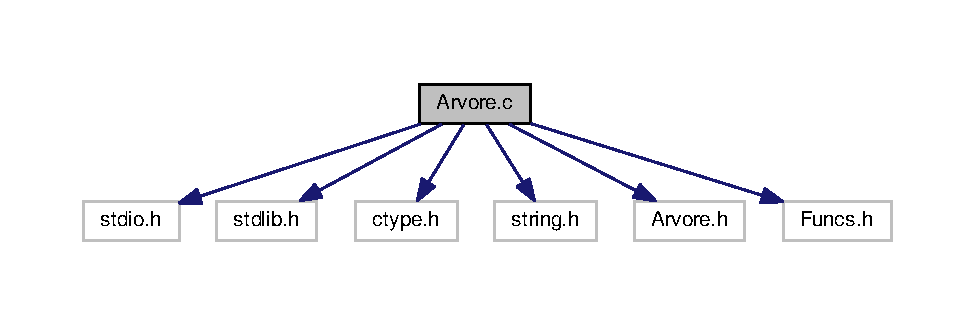
\includegraphics[width=350pt]{Arvore_8c__incl}
\end{center}
\end{figure}
\subsection*{Definições e Macros}
\begin{DoxyCompactItemize}
\item 
\#define \hyperlink{Arvore_8c_aa9c92c11eef6b6d98a1a444302093ca5}{\+\_\+\+Primary\+\_\+libraries}\hypertarget{Arvore_8c_aa9c92c11eef6b6d98a1a444302093ca5}{}\label{Arvore_8c_aa9c92c11eef6b6d98a1a444302093ca5}

\begin{DoxyCompactList}\small\item\em Header de funções padrão, para I/O, manipulação de strings. \end{DoxyCompactList}\item 
\#define \hyperlink{Arvore_8c_ad3059c7e862e1f571f036f8edbec268e}{\+\_\+\+Arvore\+\_\+library}\hypertarget{Arvore_8c_ad3059c7e862e1f571f036f8edbec268e}{}\label{Arvore_8c_ad3059c7e862e1f571f036f8edbec268e}

\begin{DoxyCompactList}\small\item\em Header da biblioteca de arvore. \end{DoxyCompactList}\item 
\#define \hyperlink{Arvore_8c_aada0c2263d9b6d55cbf5b649bc72a64a}{\+\_\+\+Funcs\+\_\+library}\hypertarget{Arvore_8c_aada0c2263d9b6d55cbf5b649bc72a64a}{}\label{Arvore_8c_aada0c2263d9b6d55cbf5b649bc72a64a}

\begin{DoxyCompactList}\small\item\em Header da biblioteca de funções (criação de arquivo e concatenação de strings). \end{DoxyCompactList}\end{DoxyCompactItemize}
\subsection*{Funções}
\begin{DoxyCompactItemize}
\item 
void \hyperlink{Arvore_8c_a11bdc8462ac661708ec7dfc6209ad039}{Constroi\+\_\+\+Manual} (arvore $\ast$$\ast$ainicio, char $\ast$no, int size)
\begin{DoxyCompactList}\small\item\em Função de criação da arvore de forma manual. \end{DoxyCompactList}\item 
void \hyperlink{Arvore_8c_a1d91a898045686dcc35f0201643fd047}{Constroi\+\_\+\+T\+XT} (arvore $\ast$$\ast$ainicio, F\+I\+LE $\ast$arq)
\begin{DoxyCompactList}\small\item\em Função de criação da arvore por .txt. \end{DoxyCompactList}\item 
void \hyperlink{Arvore_8c_a84ece5fc9e1f4d2f169800dd5f32b078}{Salva\+\_\+\+T\+XT} (arvore $\ast$$\ast$ainicio, F\+I\+LE $\ast$arq)
\begin{DoxyCompactList}\small\item\em Função para salvar as perguntas da arvore em um .txt. \end{DoxyCompactList}\item 
void \hyperlink{Arvore_8c_ab7a6f0fdd0836b340bbad8c859b16dc4}{Le} (arvore $\ast$a1)
\begin{DoxyCompactList}\small\item\em Função para a leitura da pergunta no nó da Arvore. \end{DoxyCompactList}\item 
void \hyperlink{Arvore_8c_a1f19223608412f84ebe5001d5cd539b3}{Navega\+Sim} (arvore $\ast$$\ast$pergunta)
\begin{DoxyCompactList}\small\item\em Função para a navegação e leitura da pergunta para o nó \textquotesingle{}sim\textquotesingle{} da arvore. \end{DoxyCompactList}\item 
void \hyperlink{Arvore_8c_a25ee1248463373bfb62fc366a93af84e}{Navega\+Nao} (arvore $\ast$$\ast$pergunta)
\begin{DoxyCompactList}\small\item\em Função para a navegação e leitura da pergunta para o nó \textquotesingle{}nao\textquotesingle{} da arvore. \end{DoxyCompactList}\item 
void \hyperlink{Arvore_8c_ad33c2e638a0cc3819525d8cef7119cdb}{Desconstroi} (arvore $\ast$$\ast$ainicio)
\begin{DoxyCompactList}\small\item\em Função para apagar a arvore da memória. \end{DoxyCompactList}\end{DoxyCompactItemize}


\subsection{Descrição Detalhada}
Arquivo que contem a biblioteca de manipulação e criação da arvore. 

\begin{DoxyAuthor}{Autor}
Andre Garrido Damaceno Como esse arquivo contem a biblioteca da arvore, necessita dos headers padrões e de de funções auxiliares. 
\end{DoxyAuthor}


\subsection{Funções}
\index{Arvore.\+c@{Arvore.\+c}!Constroi\+\_\+\+Manual@{Constroi\+\_\+\+Manual}}
\index{Constroi\+\_\+\+Manual@{Constroi\+\_\+\+Manual}!Arvore.\+c@{Arvore.\+c}}
\subsubsection[{\texorpdfstring{Constroi\+\_\+\+Manual(arvore $\ast$$\ast$ainicio, char $\ast$no, int size)}{Constroi_Manual(arvore **ainicio, char *no, int size)}}]{\setlength{\rightskip}{0pt plus 5cm}void Constroi\+\_\+\+Manual (
\begin{DoxyParamCaption}
\item[{arvore $\ast$$\ast$}]{ainicio, }
\item[{char $\ast$}]{no, }
\item[{int}]{size}
\end{DoxyParamCaption}
)}\hypertarget{Arvore_8c_a11bdc8462ac661708ec7dfc6209ad039}{}\label{Arvore_8c_a11bdc8462ac661708ec7dfc6209ad039}


Função de criação da arvore de forma manual. 

Essa função recebe como parametro o endereço de um ponteiro de arvore \textquotesingle{}arvore $\ast$$\ast$ainicio\textquotesingle{} (para sua criação), uma string \textquotesingle{}char $\ast$no\textquotesingle{} para a informação a respeito do nó atual para o usuário, um inteiro \textquotesingle{}int size\textquotesingle{}, para impedir a criação de mais que 20 níveis de perguntas (para garantir que o usuário poderá responder apenas 20 perguntas no máximo). A função não retorna nenhum parametro. Essa função cria a arvore de acordo com as perguntas inseridas pelo usuário, sendo possível o usuário criar quantas perguntas quiser (com o limite de 1048576 perguntas), podendo parar de inserir quando quiser. Caso haja erro de alocação de memória em \textquotesingle{}Constroi\+\_\+\+Manual\textquotesingle{} ou nas funções que ela chama, o programa é encerrado com erro. \index{Arvore.\+c@{Arvore.\+c}!Constroi\+\_\+\+T\+XT@{Constroi\+\_\+\+T\+XT}}
\index{Constroi\+\_\+\+T\+XT@{Constroi\+\_\+\+T\+XT}!Arvore.\+c@{Arvore.\+c}}
\subsubsection[{\texorpdfstring{Constroi\+\_\+\+T\+X\+T(arvore $\ast$$\ast$ainicio, F\+I\+L\+E $\ast$arq)}{Constroi_TXT(arvore **ainicio, FILE *arq)}}]{\setlength{\rightskip}{0pt plus 5cm}void Constroi\+\_\+\+T\+XT (
\begin{DoxyParamCaption}
\item[{arvore $\ast$$\ast$}]{ainicio, }
\item[{F\+I\+LE $\ast$}]{arq}
\end{DoxyParamCaption}
)}\hypertarget{Arvore_8c_a1d91a898045686dcc35f0201643fd047}{}\label{Arvore_8c_a1d91a898045686dcc35f0201643fd047}


Função de criação da arvore por .txt. 

Essa função recebe como parametro o endereço de um ponteiro de arvore \textquotesingle{}arvore $\ast$$\ast$ainicio\textquotesingle{} (para sua criação) e um arquivo (para a leitura das perguntas e criação da arvore). A função não retorna nenhum parametro. Essa função cria a arvore de acordo com um arquivo de texto aberto pelo usuário, sendo os nós nulos identificados por pontos \textquotesingle{}.\textquotesingle{}. Caso haja erro de alocação de memória em \textquotesingle{}Constroi\+\_\+\+T\+XT\textquotesingle{} o programa é encerrado com erro. \index{Arvore.\+c@{Arvore.\+c}!Desconstroi@{Desconstroi}}
\index{Desconstroi@{Desconstroi}!Arvore.\+c@{Arvore.\+c}}
\subsubsection[{\texorpdfstring{Desconstroi(arvore $\ast$$\ast$ainicio)}{Desconstroi(arvore **ainicio)}}]{\setlength{\rightskip}{0pt plus 5cm}void Desconstroi (
\begin{DoxyParamCaption}
\item[{arvore $\ast$$\ast$}]{ainicio}
\end{DoxyParamCaption}
)}\hypertarget{Arvore_8c_ad33c2e638a0cc3819525d8cef7119cdb}{}\label{Arvore_8c_ad33c2e638a0cc3819525d8cef7119cdb}


Função para apagar a arvore da memória. 

Essa função recebe como parametro o endereço do ponteiro da arvore \textquotesingle{}arvore $\ast$$\ast$ainicio\textquotesingle{} e não retorna nenhum parametro. A função navega recursivamente para o ultimo nó sim, em seguida o ultimo nó nao, e vai apagando a arvore. A função checa se o nó é N\+U\+LL, para evitar erros e conseguir apagar de forma recursiva. Caso seja inserido um nó invalido não N\+U\+LL, pode ser que ocorra um erro de Seg\+Fault. \index{Arvore.\+c@{Arvore.\+c}!Le@{Le}}
\index{Le@{Le}!Arvore.\+c@{Arvore.\+c}}
\subsubsection[{\texorpdfstring{Le(arvore $\ast$a1)}{Le(arvore *a1)}}]{\setlength{\rightskip}{0pt plus 5cm}void Le (
\begin{DoxyParamCaption}
\item[{arvore $\ast$}]{a1}
\end{DoxyParamCaption}
)}\hypertarget{Arvore_8c_ab7a6f0fdd0836b340bbad8c859b16dc4}{}\label{Arvore_8c_ab7a6f0fdd0836b340bbad8c859b16dc4}


Função para a leitura da pergunta no nó da Arvore. 

Essa função recebe como parametro um ponteiro de arvore \textquotesingle{}arvore $\ast$a1\textquotesingle{}, não retorna nenhum parametro. A função apenas checa se o ponteiro é valido, caso seja, imprime na tela a pergunta. Caso o ponteiro não seja valido (N\+U\+LL), a função não faz nada (não havendo erros). \index{Arvore.\+c@{Arvore.\+c}!Navega\+Nao@{Navega\+Nao}}
\index{Navega\+Nao@{Navega\+Nao}!Arvore.\+c@{Arvore.\+c}}
\subsubsection[{\texorpdfstring{Navega\+Nao(arvore $\ast$$\ast$pergunta)}{NavegaNao(arvore **pergunta)}}]{\setlength{\rightskip}{0pt plus 5cm}void Navega\+Nao (
\begin{DoxyParamCaption}
\item[{arvore $\ast$$\ast$}]{pergunta}
\end{DoxyParamCaption}
)}\hypertarget{Arvore_8c_a25ee1248463373bfb62fc366a93af84e}{}\label{Arvore_8c_a25ee1248463373bfb62fc366a93af84e}


Função para a navegação e leitura da pergunta para o nó \textquotesingle{}nao\textquotesingle{} da arvore. 

Essa função recebe como parametro o endereço do ponteiro da arvore, e não retorna nenhum parametro. A função checa se o nó atual é valido e se o nó \textquotesingle{}nao\textquotesingle{} é valido, caso sejam, o apontador passa a apontar para o nó \textquotesingle{}nao\textquotesingle{} e a pergunta é lida. Caso em algum ponto o nó seja N\+U\+LL, a função não faz nada, apenas retorna. \index{Arvore.\+c@{Arvore.\+c}!Navega\+Sim@{Navega\+Sim}}
\index{Navega\+Sim@{Navega\+Sim}!Arvore.\+c@{Arvore.\+c}}
\subsubsection[{\texorpdfstring{Navega\+Sim(arvore $\ast$$\ast$pergunta)}{NavegaSim(arvore **pergunta)}}]{\setlength{\rightskip}{0pt plus 5cm}void Navega\+Sim (
\begin{DoxyParamCaption}
\item[{arvore $\ast$$\ast$}]{pergunta}
\end{DoxyParamCaption}
)}\hypertarget{Arvore_8c_a1f19223608412f84ebe5001d5cd539b3}{}\label{Arvore_8c_a1f19223608412f84ebe5001d5cd539b3}


Função para a navegação e leitura da pergunta para o nó \textquotesingle{}sim\textquotesingle{} da arvore. 

Essa função recebe como parametro o endereço do ponteiro da arvore, e não retorna nenhum parametro. A função checa se o nó atual é valido e se o nó \textquotesingle{}sim\textquotesingle{} é valido, caso sejam, o apontador passa a apontar para o nó \textquotesingle{}sim\textquotesingle{} e a pergunta é lida. Caso em algum ponto o nó seja N\+U\+LL, a função não faz nada, apenas retorna. \index{Arvore.\+c@{Arvore.\+c}!Salva\+\_\+\+T\+XT@{Salva\+\_\+\+T\+XT}}
\index{Salva\+\_\+\+T\+XT@{Salva\+\_\+\+T\+XT}!Arvore.\+c@{Arvore.\+c}}
\subsubsection[{\texorpdfstring{Salva\+\_\+\+T\+X\+T(arvore $\ast$$\ast$ainicio, F\+I\+L\+E $\ast$arq)}{Salva_TXT(arvore **ainicio, FILE *arq)}}]{\setlength{\rightskip}{0pt plus 5cm}void Salva\+\_\+\+T\+XT (
\begin{DoxyParamCaption}
\item[{arvore $\ast$$\ast$}]{ainicio, }
\item[{F\+I\+LE $\ast$}]{arq}
\end{DoxyParamCaption}
)}\hypertarget{Arvore_8c_a84ece5fc9e1f4d2f169800dd5f32b078}{}\label{Arvore_8c_a84ece5fc9e1f4d2f169800dd5f32b078}


Função para salvar as perguntas da arvore em um .txt. 

Essa função recebe como parametro o endereço do ponteiro de uma arvore \textquotesingle{}arvore $\ast$$\ast$ainicio\textquotesingle{}, e o arquivo de texto a ser salvo as perguntas da arvore \textquotesingle{}F\+I\+LE $\ast$arq\textquotesingle{}. A função não retorna nenhum parametro. A função salva a pergunta no arquivo .txt, caso o nó seja N\+U\+LL, é salvo um \textquotesingle{}.\textquotesingle{} no arquivo. Caso o arquivo seja inexistente, a função não faz nada. Caso a arvore seja inexistente, a função salva apenas um \textquotesingle{}.\textquotesingle{} no .txt (não havendo erros). 
\hypertarget{Funcs_8c}{}\section{Referência do Arquivo Funcs.\+c}
\label{Funcs_8c}\index{Funcs.\+c@{Funcs.\+c}}


Arquivo que contem a função de concatenação de string e de criar arquivos txt (abrir ou salvar).  


{\ttfamily \#include $<$stdio.\+h$>$}\\*
{\ttfamily \#include $<$stdlib.\+h$>$}\\*
{\ttfamily \#include $<$ctype.\+h$>$}\\*
{\ttfamily \#include $<$string.\+h$>$}\\*
{\ttfamily \#include $<$assert.\+h$>$}\\*
{\ttfamily \#include \char`\"{}Funcs.\+h\char`\"{}}\\*
Gráfico de dependência de inclusões para Funcs.\+c\+:\nopagebreak
\begin{figure}[H]
\begin{center}
\leavevmode
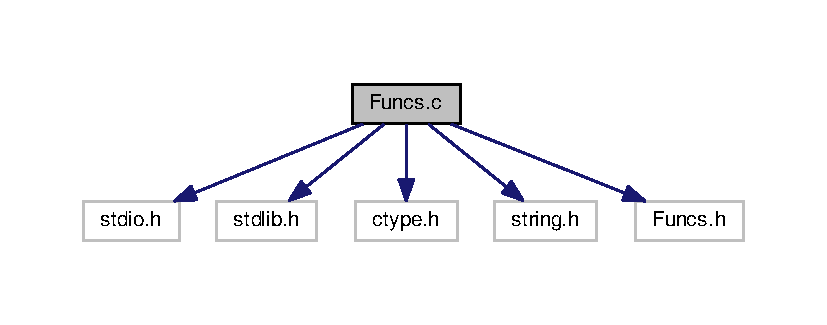
\includegraphics[width=350pt]{Funcs_8c__incl}
\end{center}
\end{figure}
\subsection*{Definições e Macros}
\begin{DoxyCompactItemize}
\item 
\#define \hyperlink{Funcs_8c_aa9c92c11eef6b6d98a1a444302093ca5}{\+\_\+\+Primary\+\_\+libraries}
\begin{DoxyCompactList}\small\item\em Header de funções padrão, para I/O, manipulação de strings. \end{DoxyCompactList}\item 
\#define \hyperlink{Funcs_8c_aada0c2263d9b6d55cbf5b649bc72a64a}{\+\_\+\+Funcs\+\_\+library}\hypertarget{Funcs_8c_aada0c2263d9b6d55cbf5b649bc72a64a}{}\label{Funcs_8c_aada0c2263d9b6d55cbf5b649bc72a64a}

\begin{DoxyCompactList}\small\item\em Header da biblioteca de funções (criação de arquivo e concatenação de strings). \end{DoxyCompactList}\end{DoxyCompactItemize}
\subsection*{Funções}
\begin{DoxyCompactItemize}
\item 
F\+I\+LE $\ast$ \hyperlink{Funcs_8c_ae514617a2ce835b9ba8c3974e6e09f3b}{Cria\+Arquivo} (char $\ast$type, char $\ast$opcao)
\begin{DoxyCompactList}\small\item\em Função de Criação de arquivos (abertura ou leitura). \end{DoxyCompactList}\item 
char $\ast$ \hyperlink{Funcs_8c_ab6e869105db05a7a2253c50108cb8583}{Constroi\+No} (char $\ast$no, char $\ast$filho)
\begin{DoxyCompactList}\small\item\em Função de concatenação de string. \end{DoxyCompactList}\end{DoxyCompactItemize}


\subsection{Descrição Detalhada}
Arquivo que contem a função de concatenação de string e de criar arquivos txt (abrir ou salvar). 

\begin{DoxyAuthor}{Autor}
Andre Garrido Damaceno 
\end{DoxyAuthor}


\subsection{Definições e macros}
\index{Funcs.\+c@{Funcs.\+c}!\+\_\+\+Primary\+\_\+libraries@{\+\_\+\+Primary\+\_\+libraries}}
\index{\+\_\+\+Primary\+\_\+libraries@{\+\_\+\+Primary\+\_\+libraries}!Funcs.\+c@{Funcs.\+c}}
\subsubsection[{\texorpdfstring{\+\_\+\+Primary\+\_\+libraries}{_Primary_libraries}}]{\setlength{\rightskip}{0pt plus 5cm}\#define \+\_\+\+Primary\+\_\+libraries}\hypertarget{Funcs_8c_aa9c92c11eef6b6d98a1a444302093ca5}{}\label{Funcs_8c_aa9c92c11eef6b6d98a1a444302093ca5}


Header de funções padrão, para I/O, manipulação de strings. 

Como esse arquivo contem apenas funções auxiliares, necessita apenas dos headers padrões. 

\subsection{Funções}
\index{Funcs.\+c@{Funcs.\+c}!Constroi\+No@{Constroi\+No}}
\index{Constroi\+No@{Constroi\+No}!Funcs.\+c@{Funcs.\+c}}
\subsubsection[{\texorpdfstring{Constroi\+No(char $\ast$no, char $\ast$filho)}{ConstroiNo(char *no, char *filho)}}]{\setlength{\rightskip}{0pt plus 5cm}char$\ast$ Constroi\+No (
\begin{DoxyParamCaption}
\item[{char $\ast$}]{no, }
\item[{char $\ast$}]{filho}
\end{DoxyParamCaption}
)}\hypertarget{Funcs_8c_ab6e869105db05a7a2253c50108cb8583}{}\label{Funcs_8c_ab6e869105db05a7a2253c50108cb8583}


Função de concatenação de string. 

Parametros\+: Essa função recebe como parametro duas strings \textquotesingle{}char $\ast$no\textquotesingle{} e \textquotesingle{}char $\ast$filho\textquotesingle{}, concatena a string \textquotesingle{}filho\textquotesingle{} na string \textquotesingle{}no\textquotesingle{}, e retorna essa string \textquotesingle{}char $\ast$\textquotesingle{}.

Tratamento de erros\+: Caso o computador negue a alocação de memória, o programa é finalizado.

Descrição\+: Inicialmente a função aloca memória suficiente para a concatenação das strings, em seguida copia a string \textquotesingle{}no\textquotesingle{} para a memoria alocada, por fim, concatena a string \textquotesingle{}filho\textquotesingle{} na memoria alocada, retornando assim a string com \textquotesingle{}no\textquotesingle{} e \textquotesingle{}filho\textquotesingle{} concatenados devidamente.

Assertivas de entrada\+: As strings \textquotesingle{}no\textquotesingle{} e \textquotesingle{}filho\textquotesingle{} não podem ser N\+U\+L\+Ls.

Requisitos\+: A função deve concatenar as duas strings recebidas \textquotesingle{}no\textquotesingle{} e \textquotesingle{}filho\textquotesingle{} e retornar a string concatenada.

Hipoteses\+: A função aloca devidamente memória suficiente para a string final concatenada, e faz a concatenação de forma correta, concatenando no sentido \textquotesingle{}no\textquotesingle{} e \textquotesingle{}filho\textquotesingle{}.

Assertivas de saida\+: A string com o resultado da concatenação não deve ser N\+U\+LL, O tamanho da string retornada deve ser o tamanho de \textquotesingle{}no\textquotesingle{} + \textquotesingle{}filho\textquotesingle{}, e o final da string deve conter o caracter \textquotesingle{}\textbackslash{}0\textquotesingle{}.

Interface explicita\+:

Interface implicita\+:

Contrato na especificação\+: A função deve receber duas strings \textquotesingle{}no\textquotesingle{} e \textquotesingle{}filho\textquotesingle{} não nulas, deve então alocar uma nova string \textquotesingle{}no\+Filho\textquotesingle{} que deve possuir o tamanho de \textquotesingle{}no\textquotesingle{} e \textquotesingle{}filho\textquotesingle{} juntas, em seguida colocar o resultado da concatenação de \textquotesingle{}no\textquotesingle{} e \textquotesingle{}filho\textquotesingle{} em \textquotesingle{}no\+Filho\textquotesingle{} e retornar \textquotesingle{}no\+Filho\textquotesingle{}. \index{Funcs.\+c@{Funcs.\+c}!Cria\+Arquivo@{Cria\+Arquivo}}
\index{Cria\+Arquivo@{Cria\+Arquivo}!Funcs.\+c@{Funcs.\+c}}
\subsubsection[{\texorpdfstring{Cria\+Arquivo(char $\ast$type, char $\ast$opcao)}{CriaArquivo(char *type, char *opcao)}}]{\setlength{\rightskip}{0pt plus 5cm}F\+I\+LE$\ast$ Cria\+Arquivo (
\begin{DoxyParamCaption}
\item[{char $\ast$}]{type, }
\item[{char $\ast$}]{opcao}
\end{DoxyParamCaption}
)}\hypertarget{Funcs_8c_ae514617a2ce835b9ba8c3974e6e09f3b}{}\label{Funcs_8c_ae514617a2ce835b9ba8c3974e6e09f3b}


Função de Criação de arquivos (abertura ou leitura). 

Parametros\+: Essa função recebe como parametro o tipo de abertura \textquotesingle{}char $\ast$type\textquotesingle{} (\char`\"{}r\char`\"{} -\/ para read, \char`\"{}w\char`\"{} -\/ para write) e também uma string \textquotesingle{}char $\ast$opcao\textquotesingle{} para ser impresso na tela (informando ao usuário se o arquivo esta sendo aberto ou salvo). A função retorna o arquivo \textquotesingle{}F\+I\+LE $\ast$\textquotesingle{}.

Tratamento de erros\+: Caso o arquivo não exista, ou ele será criado (no caso do tipo \char`\"{}w\char`\"{} -\/ write), ou a função retornará N\+U\+LL no \textquotesingle{}F\+I\+LE $\ast$\textquotesingle{}.

Descrição\+: Essa função apenas abre um arquivo e o retorna para o usuário.

Assertivas de entrada\+: string \textquotesingle{}type\textquotesingle{} e \textquotesingle{}opcao\textquotesingle{} não N\+U\+L\+Ls.

Requisitos\+: A função deve perguntar ao usuário qual o nome do arquivo e abrir ou criar um arquivo de acordo com o parâmetro \textquotesingle{}type\textquotesingle{}.

Hipoteses\+: A função deve abrir o arquivo de forma adequada de acordo com a forma de abertura \textquotesingle{}type\textquotesingle{} requisitado, retornando o arquivos aberto/criado.

Assertivas de saida\+: Arquivo aberto/criado não ser N\+UL

Interface explicita\+:

Interface implicita\+:

Contrato na especificação\+: A função deve receber a forma de abertura/criação do arquivo \textquotesingle{}type\textquotesingle{}, e uma string com a informação para o usuário do que está ocorrendo. Então, deve ser aberto/criado o arquivo de acordo com o parâmetro \textquotesingle{}type\textquotesingle{} e o nome informado pelo usuário, e por fim, deve ser retornado o arquivo. 
\hypertarget{Jogo_8c}{}\section{Referência do Arquivo Jogo.\+c}
\label{Jogo_8c}\index{Jogo.\+c@{Jogo.\+c}}


Arquivo que contem a Main e uma função de chamadas para executar o jogo.  


{\ttfamily \#include $<$stdio.\+h$>$}\\*
{\ttfamily \#include $<$stdlib.\+h$>$}\\*
{\ttfamily \#include $<$ctype.\+h$>$}\\*
{\ttfamily \#include $<$string.\+h$>$}\\*
{\ttfamily \#include \char`\"{}Arvore.\+h\char`\"{}}\\*
{\ttfamily \#include \char`\"{}Funcs.\+h\char`\"{}}\\*
{\ttfamily \#include \char`\"{}Vinte\+\_\+\+Perguntas.\+h\char`\"{}}\\*
{\ttfamily \#include \char`\"{}Jogo.\+h\char`\"{}}\\*
Gráfico de dependência de inclusões para Jogo.\+c\+:\nopagebreak
\begin{figure}[H]
\begin{center}
\leavevmode
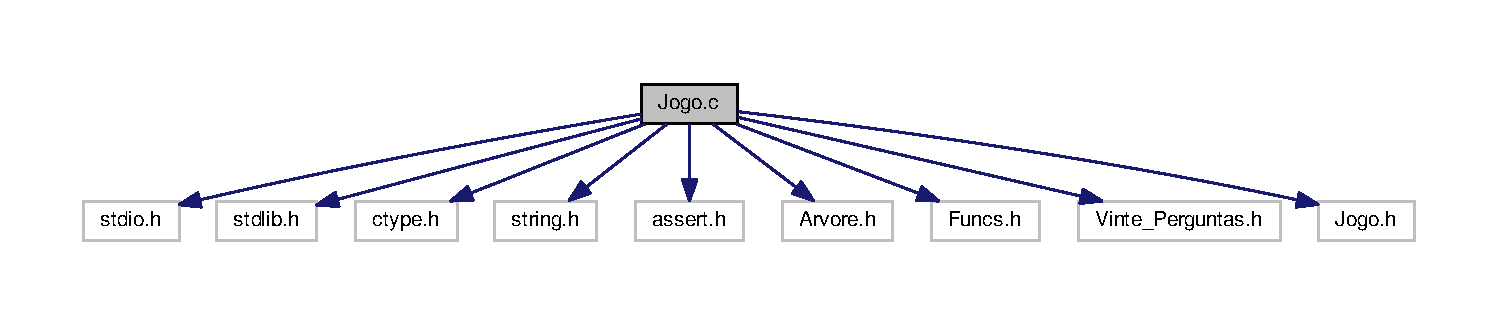
\includegraphics[width=350pt]{Jogo_8c__incl}
\end{center}
\end{figure}
\subsection*{Definições e Macros}
\begin{DoxyCompactItemize}
\item 
\#define \hyperlink{Jogo_8c_aa9c92c11eef6b6d98a1a444302093ca5}{\+\_\+\+Primary\+\_\+libraries}
\begin{DoxyCompactList}\small\item\em Header de funções padrão, para I/O, manipulação de strings. \end{DoxyCompactList}\item 
\#define \hyperlink{Jogo_8c_ad3059c7e862e1f571f036f8edbec268e}{\+\_\+\+Arvore\+\_\+library}\hypertarget{Jogo_8c_ad3059c7e862e1f571f036f8edbec268e}{}\label{Jogo_8c_ad3059c7e862e1f571f036f8edbec268e}

\begin{DoxyCompactList}\small\item\em Header da biblioteca de arvore. \end{DoxyCompactList}\item 
\#define \hyperlink{Jogo_8c_aada0c2263d9b6d55cbf5b649bc72a64a}{\+\_\+\+Funcs\+\_\+library}\hypertarget{Jogo_8c_aada0c2263d9b6d55cbf5b649bc72a64a}{}\label{Jogo_8c_aada0c2263d9b6d55cbf5b649bc72a64a}

\begin{DoxyCompactList}\small\item\em Header da biblioteca de funções (criação de arquivo e concatenação de strings). \end{DoxyCompactList}\item 
\#define \hyperlink{Jogo_8c_a18fc926bd99ef27d0302ea3f50e1424e}{\+\_\+\+Vinte\+\_\+\+Perguntas\+\_\+library}\hypertarget{Jogo_8c_a18fc926bd99ef27d0302ea3f50e1424e}{}\label{Jogo_8c_a18fc926bd99ef27d0302ea3f50e1424e}

\begin{DoxyCompactList}\small\item\em Header da biblioteca de estruturação (execução) do jogo de 20 perguntas. \end{DoxyCompactList}\item 
\#define \hyperlink{Jogo_8c_a22dc5c94c24cf28b5260af7777f0bb1b}{\+\_\+\+Jogo\+\_\+library}\hypertarget{Jogo_8c_a22dc5c94c24cf28b5260af7777f0bb1b}{}\label{Jogo_8c_a22dc5c94c24cf28b5260af7777f0bb1b}

\begin{DoxyCompactList}\small\item\em Header da biblioteca que inicializa o jogo. \end{DoxyCompactList}\end{DoxyCompactItemize}
\subsection*{Funções}
\begin{DoxyCompactItemize}
\item 
int \hyperlink{Jogo_8c_ae66f6b31b5ad750f1fe042a706a4e3d4}{main} ()
\begin{DoxyCompactList}\small\item\em Main de inicialização do jogo. \end{DoxyCompactList}\item 
void \hyperlink{Jogo_8c_aa95326e6eb7941a743d5543f82d7c7de}{Jogo\+\_\+init} (void)
\begin{DoxyCompactList}\small\item\em Função de inicialização do jogo. \end{DoxyCompactList}\end{DoxyCompactItemize}


\subsection{Descrição Detalhada}
Arquivo que contem a Main e uma função de chamadas para executar o jogo. 

\begin{DoxyAuthor}{Autor}
Andre Garrido Damaceno 
\end{DoxyAuthor}


\subsection{Definições e macros}
\index{Jogo.\+c@{Jogo.\+c}!\+\_\+\+Primary\+\_\+libraries@{\+\_\+\+Primary\+\_\+libraries}}
\index{\+\_\+\+Primary\+\_\+libraries@{\+\_\+\+Primary\+\_\+libraries}!Jogo.\+c@{Jogo.\+c}}
\subsubsection[{\texorpdfstring{\+\_\+\+Primary\+\_\+libraries}{_Primary_libraries}}]{\setlength{\rightskip}{0pt plus 5cm}\#define \+\_\+\+Primary\+\_\+libraries}\hypertarget{Jogo_8c_aa9c92c11eef6b6d98a1a444302093ca5}{}\label{Jogo_8c_aa9c92c11eef6b6d98a1a444302093ca5}


Header de funções padrão, para I/O, manipulação de strings. 

Como esse arquivo contem a função que inicializa o jogo, são necessários todos arquivos headers que o programa utiliza. 

\subsection{Funções}
\index{Jogo.\+c@{Jogo.\+c}!Jogo\+\_\+init@{Jogo\+\_\+init}}
\index{Jogo\+\_\+init@{Jogo\+\_\+init}!Jogo.\+c@{Jogo.\+c}}
\subsubsection[{\texorpdfstring{Jogo\+\_\+init(void)}{Jogo_init(void)}}]{\setlength{\rightskip}{0pt plus 5cm}void Jogo\+\_\+init (
\begin{DoxyParamCaption}
\item[{void}]{}
\end{DoxyParamCaption}
)}\hypertarget{Jogo_8c_aa95326e6eb7941a743d5543f82d7c7de}{}\label{Jogo_8c_aa95326e6eb7941a743d5543f82d7c7de}


Função de inicialização do jogo. 

A função não recebe nem retorna nenhum parâmentro. Nessa função, primeiramente é populado os dados na arvore (por arquivo de texto ou por criação manual). Em seguida, inicializa-\/se o jogo ao chamar a função \textquotesingle{}\hyperlink{Vinte__Perguntas_8c_a50cd5030c633ddd0c6cc9bcfb9adfd88}{Vinte\+\_\+\+Perguntas()}\textquotesingle{}, ao fim, é perguntado ao usuário se quer salvar os dados de seu jogo em um arquivo .txt, e por fim é finalizada a execução (deletando a arvore da memoria). Caso haja algum erro em alocação de memória, o programa é encerrado. Outros casos variam, caso a arvore seja null, eventualmente havera a opção de tentar recriar a arvore. Caso haja algum outro erro totalmente imprevisto, ou as funções internas o conterão, ou o programa finalizará com erro.

Assertivas de entrada\+:

Requisitos\+:

Hipoteses\+:

Assertivas de saida\+:

Interface explicita\+:

Interface implicita\+:

Contrato na especificação\+: \index{Jogo.\+c@{Jogo.\+c}!main@{main}}
\index{main@{main}!Jogo.\+c@{Jogo.\+c}}
\subsubsection[{\texorpdfstring{main()}{main()}}]{\setlength{\rightskip}{0pt plus 5cm}int main (
\begin{DoxyParamCaption}
{}
\end{DoxyParamCaption}
)}\hypertarget{Jogo_8c_ae66f6b31b5ad750f1fe042a706a4e3d4}{}\label{Jogo_8c_ae66f6b31b5ad750f1fe042a706a4e3d4}


Main de inicialização do jogo. 

A main apenas chama a função de inicialização \textquotesingle{}\hyperlink{Jogo_8c_aa95326e6eb7941a743d5543f82d7c7de}{Jogo\+\_\+init()}\textquotesingle{}, que chama as funções do jogo em ordem lógica para sua execução normal.

Assertivas de entrada\+:

Requisitos\+:

Hipoteses\+:

Assertivas de saida\+:

Interface explicita\+:

Interface implicita\+:

Contrato na especificação\+: 
\hypertarget{Testa__Arvore_8cpp}{}\section{Referência do Arquivo Testa\+\_\+\+Arvore.\+cpp}
\label{Testa__Arvore_8cpp}\index{Testa\+\_\+\+Arvore.\+cpp@{Testa\+\_\+\+Arvore.\+cpp}}


Arquivo que contem os testes do jogo de 20 perguntas.  


{\ttfamily \#include \char`\"{}catch.\+hpp\char`\"{}}\\*
{\ttfamily \#include \char`\"{}Arvore.\+h\char`\"{}}\\*
{\ttfamily \#include \char`\"{}Funcs.\+h\char`\"{}}\\*
{\ttfamily \#include \char`\"{}Vinte\+\_\+\+Perguntas.\+h\char`\"{}}\\*
Gráfico de dependência de inclusões para Testa\+\_\+\+Arvore.\+cpp\+:\nopagebreak
\begin{figure}[H]
\begin{center}
\leavevmode
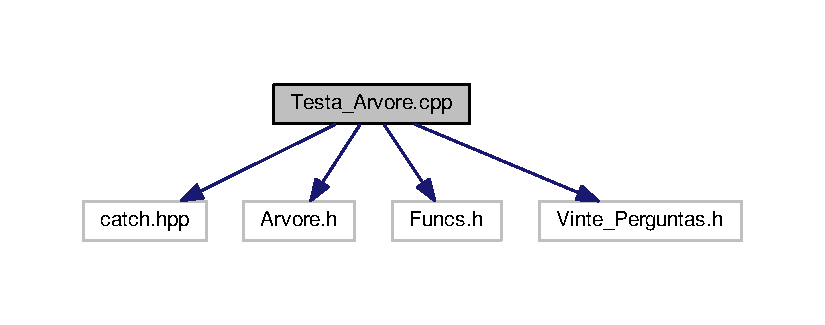
\includegraphics[width=350pt]{Testa__Arvore_8cpp__incl}
\end{center}
\end{figure}
\subsection*{Definições e Macros}
\begin{DoxyCompactItemize}
\item 
\#define \hyperlink{Testa__Arvore_8cpp_a656eb5868e824d59f489f910db438420}{C\+A\+T\+C\+H\+\_\+\+C\+O\+N\+F\+I\+G\+\_\+\+M\+A\+IN}
\item 
\#define \hyperlink{Testa__Arvore_8cpp_ab4b7ceac16a6ea2999b93f42d7a9b638}{\+\_\+\+Catch}\hypertarget{Testa__Arvore_8cpp_ab4b7ceac16a6ea2999b93f42d7a9b638}{}\label{Testa__Arvore_8cpp_ab4b7ceac16a6ea2999b93f42d7a9b638}

\begin{DoxyCompactList}\small\item\em Header da biblioteca de testes. \end{DoxyCompactList}\item 
\#define \hyperlink{Testa__Arvore_8cpp_ad3059c7e862e1f571f036f8edbec268e}{\+\_\+\+Arvore\+\_\+library}\hypertarget{Testa__Arvore_8cpp_ad3059c7e862e1f571f036f8edbec268e}{}\label{Testa__Arvore_8cpp_ad3059c7e862e1f571f036f8edbec268e}

\begin{DoxyCompactList}\small\item\em Header da biblioteca de arvore. \end{DoxyCompactList}\item 
\#define \hyperlink{Testa__Arvore_8cpp_aada0c2263d9b6d55cbf5b649bc72a64a}{\+\_\+\+Funcs\+\_\+library}\hypertarget{Testa__Arvore_8cpp_aada0c2263d9b6d55cbf5b649bc72a64a}{}\label{Testa__Arvore_8cpp_aada0c2263d9b6d55cbf5b649bc72a64a}

\begin{DoxyCompactList}\small\item\em Header da biblioteca de funções (criação de arquivo e concatenação de strings). \end{DoxyCompactList}\item 
\#define \hyperlink{Testa__Arvore_8cpp_a18fc926bd99ef27d0302ea3f50e1424e}{\+\_\+\+Vinte\+\_\+\+Perguntas\+\_\+library}\hypertarget{Testa__Arvore_8cpp_a18fc926bd99ef27d0302ea3f50e1424e}{}\label{Testa__Arvore_8cpp_a18fc926bd99ef27d0302ea3f50e1424e}

\begin{DoxyCompactList}\small\item\em Header da biblioteca de estruturação (execução) do jogo de 20 perguntas. \end{DoxyCompactList}\end{DoxyCompactItemize}
\subsection*{Funções}
\begin{DoxyCompactItemize}
\item 
\hyperlink{Testa__Arvore_8cpp_a08a49c56066daf348a84d92832092ee1}{T\+E\+S\+T\+\_\+\+C\+A\+SE} (\char`\"{}Creating a tree from user input\char`\"{},\char`\"{}Prove that the tree is created\char`\"{})
\begin{DoxyCompactList}\small\item\em Teste da função \textquotesingle{}Constroi\+\_\+\+Manual\textquotesingle{}. \end{DoxyCompactList}\item 
\hyperlink{Testa__Arvore_8cpp_aae0dc9964263481842ca5c93ee639022}{T\+E\+S\+T\+\_\+\+C\+A\+SE} (\char`\"{}Creating a tree from a file\char`\"{},\char`\"{}Prove that the tree is created\char`\"{})
\begin{DoxyCompactList}\small\item\em Testes da função \textquotesingle{}Constroi\+\_\+\+T\+XT\textquotesingle{} -\/ Criação normal da arvore. \end{DoxyCompactList}\item 
\hyperlink{Testa__Arvore_8cpp_a30a1f60b8f711329fc88b50af1eacc03}{T\+E\+S\+T\+\_\+\+C\+A\+SE} (\char`\"{}Trying to create a tree from an non existing file\char`\"{},\char`\"{}Prove that the tree is not created\char`\"{})
\begin{DoxyCompactList}\small\item\em Testes da função \textquotesingle{}Constroi\+\_\+\+T\+XT\textquotesingle{} -\/ tentativa de criar arvore por arquivo Null. \end{DoxyCompactList}\item 
\hyperlink{Testa__Arvore_8cpp_a9d22244470a4cc23b7c975f5ad5df612}{T\+E\+S\+T\+\_\+\+C\+A\+SE} (\char`\"{}Trying to navigate to save a N\+U\+LL tree to file\char`\"{},\char`\"{}Prove that the txt saves \textquotesingle{}.\textquotesingle{}\char`\"{})
\begin{DoxyCompactList}\small\item\em Testes da função \textquotesingle{}Salva\+\_\+\+T\+XT\textquotesingle{} -\/ tentativa de salvar arvore N\+U\+LL. \end{DoxyCompactList}\item 
\hyperlink{Testa__Arvore_8cpp_a89fc4bda1a6422a093210d0a4324a5ee}{T\+E\+S\+T\+\_\+\+C\+A\+SE} (\char`\"{}Saving a tree to file\char`\"{},\char`\"{}Prove that the txt saves the tree\char`\"{})
\begin{DoxyCompactList}\small\item\em Testes da função \textquotesingle{}Salva\+\_\+\+T\+XT\textquotesingle{} -\/ tentativa de salvar arvore existente. \end{DoxyCompactList}\item 
\hyperlink{Testa__Arvore_8cpp_ae68681daf9290cc2f69a0cb91a9173df}{T\+E\+S\+T\+\_\+\+C\+A\+SE} (\char`\"{}Saving tree to N\+U\+LL file\char`\"{},\char`\"{}Prove that the function does nothing and contains the program\char`\"{})
\begin{DoxyCompactList}\small\item\em Testes da função \textquotesingle{}Salva\+\_\+\+T\+XT\textquotesingle{} -\/ tentativa de salvar arquivo inexistente. \end{DoxyCompactList}\item 
\hyperlink{Testa__Arvore_8cpp_ae429578c484b993cb0639844d6eb213c}{T\+E\+S\+T\+\_\+\+C\+A\+SE} (\char`\"{}Freeing an existing tree\char`\"{},\char`\"{}the tree is freed\char`\"{})
\begin{DoxyCompactList}\small\item\em Teste da função \textquotesingle{}Desconstroi\textquotesingle{} -\/ Apagando uma arvore existente. \end{DoxyCompactList}\item 
\hyperlink{Testa__Arvore_8cpp_ad52052c336d92e3201f52ce8acd225d1}{T\+E\+S\+T\+\_\+\+C\+A\+SE} (\char`\"{}Freeing a N\+U\+LL tree\char`\"{},\char`\"{}the program is contained\char`\"{})
\begin{DoxyCompactList}\small\item\em Teste da função \textquotesingle{}Desconstroi\textquotesingle{} -\/ Apagando uma arvore inexistente. \end{DoxyCompactList}\item 
\hyperlink{Testa__Arvore_8cpp_a59de4e65331b095e8163209825ca73ad}{T\+E\+S\+T\+\_\+\+C\+A\+SE} (\char`\"{}Reading a tree question\char`\"{},\char`\"{}tree is unmodified and question is read\char`\"{})
\begin{DoxyCompactList}\small\item\em Teste da função Le -\/ lendo arvore existente. \end{DoxyCompactList}\item 
\hyperlink{Testa__Arvore_8cpp_a2cc69249e8bcba153203c611664fc490}{T\+E\+S\+T\+\_\+\+C\+A\+SE} (\char`\"{}Trying to read N\+U\+LL tree\char`\"{},\char`\"{}Program is contained and function does nothing\char`\"{})
\begin{DoxyCompactList}\small\item\em Teste da função Le -\/ lendo arvore inexistente. \end{DoxyCompactList}\item 
\hyperlink{Testa__Arvore_8cpp_a78c16933a4792de2cf02a5c402ee21be}{T\+E\+S\+T\+\_\+\+C\+A\+SE} (\char`\"{}Trying to navigate to \textquotesingle{}-\/$>$sim\textquotesingle{} and \textquotesingle{}-\/$>$nao\textquotesingle{} and reading the question\char`\"{},\char`\"{}Tree goes to specific navigation and reads the question\char`\"{})
\begin{DoxyCompactList}\small\item\em Testes de navegação (sim e nao) -\/ arvore existente. \end{DoxyCompactList}\item 
\hyperlink{Testa__Arvore_8cpp_a0cee031fe604571f9858f44388743016}{T\+E\+S\+T\+\_\+\+C\+A\+SE} (\char`\"{}Trying to navigate to \textquotesingle{}-\/$>$sim\textquotesingle{} and \textquotesingle{}-\/$>$nao\textquotesingle{} whith N\+U\+LL tree\char`\"{},\char`\"{}Program is contained and function returns 2\char`\"{})
\begin{DoxyCompactList}\small\item\em Testes de navegação (sim e nao) -\/ arvore inexistente. \end{DoxyCompactList}\item 
\hyperlink{Testa__Arvore_8cpp_ae555a574ec75624b4553a0a2b46cb7c6}{T\+E\+S\+T\+\_\+\+C\+A\+SE} (\char`\"{}Creating/Opening a file (read) and (write)\char`\"{},\char`\"{}Function opens/creates the file\char`\"{})
\begin{DoxyCompactList}\small\item\em Teste da função \textquotesingle{}Cria\+Arquivo\textquotesingle{} -\/ arquivos existentes \char`\"{}r\char`\"{} e \char`\"{}w\char`\"{} e arquivos inexistentes. \end{DoxyCompactList}\item 
\hyperlink{Testa__Arvore_8cpp_a488caefe9ad92a7fe27b73d1f5ab81f6}{T\+E\+S\+T\+\_\+\+C\+A\+SE} (\char`\"{}Function that concatenates strings\char`\"{},\char`\"{}Should concatenate the string\char`\"{})
\begin{DoxyCompactList}\small\item\em Testando a função \textquotesingle{}Constroi\+No\textquotesingle{} -\/ Concatenação de strings existente e inexistente. \end{DoxyCompactList}\item 
\hyperlink{Testa__Arvore_8cpp_a948870d6e9e00c16977f7d751b67403b}{T\+E\+S\+T\+\_\+\+C\+A\+SE} (\char`\"{}Testing user\textquotesingle{}s answers in game\char`\"{},\char`\"{}Get only \textquotesingle{}sim\textquotesingle{}, \textquotesingle{}nao\textquotesingle{}, \textquotesingle{}editar\textquotesingle{}, \textquotesingle{}apagar\textquotesingle{} answer and nothing else\char`\"{})
\begin{DoxyCompactList}\small\item\em Testando a função \textquotesingle{}Resposta\textquotesingle{} -\/ teste para o tipo \textquotesingle{}simples\textquotesingle{}, \textquotesingle{}multipla\textquotesingle{} e inicializacao. \end{DoxyCompactList}\item 
\hyperlink{Testa__Arvore_8cpp_a74876aec2dbe751f844d19ef08dd9aa8}{T\+E\+S\+T\+\_\+\+C\+A\+SE} (\char`\"{}Receiving null tree or object was not guessed by \hyperlink{Vinte__Perguntas_8c_a50cd5030c633ddd0c6cc9bcfb9adfd88}{Vinte\+\_\+\+Perguntas}\char`\"{},\char`\"{}The function should be contained, should ask the user to add more questions if less than 20 answers\char`\"{})
\begin{DoxyCompactList}\small\item\em Teste da função \textquotesingle{}Vinte\+\_\+\+Perguntas\textquotesingle{} -\/ Arvore inexistente. \end{DoxyCompactList}\item 
\hyperlink{Testa__Arvore_8cpp_adca0fdb9cafcd35fea4306937d1c1a08}{T\+E\+S\+T\+\_\+\+C\+A\+SE} (\char`\"{}Receiving 20 questions and testing \textquotesingle{}apagar\textquotesingle{} and \textquotesingle{}editar\textquotesingle{} in \hyperlink{Vinte__Perguntas_8c_a50cd5030c633ddd0c6cc9bcfb9adfd88}{Vinte\+\_\+\+Perguntas}\char`\"{},\char`\"{}The function should ask the questions and navigate in the tree, and execute its functions \textquotesingle{}apagar\textquotesingle{}, \textquotesingle{}editar\textquotesingle{}\char`\"{})
\begin{DoxyCompactList}\small\item\em Teste da função \textquotesingle{}Vinte\+\_\+\+Perguntas\textquotesingle{} -\/ Arvore existente, cheia, edição, apagar. \end{DoxyCompactList}\item 
\hyperlink{Testa__Arvore_8cpp_af5868ed98ec7b8f5a83b88558c4e382d}{T\+E\+S\+T\+\_\+\+C\+A\+SE} (\char`\"{}Creating childs at the end in \textquotesingle{}sim\textquotesingle{} and \textquotesingle{}nao\textquotesingle{}\char`\"{},\char`\"{}Should normaly create childs\char`\"{})
\begin{DoxyCompactList}\small\item\em Teste da função \textquotesingle{}Pergunta\+\_\+\+Final\textquotesingle{}. \end{DoxyCompactList}\end{DoxyCompactItemize}


\subsection{Descrição Detalhada}
Arquivo que contem os testes do jogo de 20 perguntas. 

\begin{DoxyAuthor}{Autor}
Andre Garrido Damaceno 
\end{DoxyAuthor}


\subsection{Definições e macros}
\index{Testa\+\_\+\+Arvore.\+cpp@{Testa\+\_\+\+Arvore.\+cpp}!C\+A\+T\+C\+H\+\_\+\+C\+O\+N\+F\+I\+G\+\_\+\+M\+A\+IN@{C\+A\+T\+C\+H\+\_\+\+C\+O\+N\+F\+I\+G\+\_\+\+M\+A\+IN}}
\index{C\+A\+T\+C\+H\+\_\+\+C\+O\+N\+F\+I\+G\+\_\+\+M\+A\+IN@{C\+A\+T\+C\+H\+\_\+\+C\+O\+N\+F\+I\+G\+\_\+\+M\+A\+IN}!Testa\+\_\+\+Arvore.\+cpp@{Testa\+\_\+\+Arvore.\+cpp}}
\subsubsection[{\texorpdfstring{C\+A\+T\+C\+H\+\_\+\+C\+O\+N\+F\+I\+G\+\_\+\+M\+A\+IN}{CATCH_CONFIG_MAIN}}]{\setlength{\rightskip}{0pt plus 5cm}\#define C\+A\+T\+C\+H\+\_\+\+C\+O\+N\+F\+I\+G\+\_\+\+M\+A\+IN}\hypertarget{Testa__Arvore_8cpp_a656eb5868e824d59f489f910db438420}{}\label{Testa__Arvore_8cpp_a656eb5868e824d59f489f910db438420}
Como esse arquivo contem os testes, necessita dos headers de toda a biblioteca do jogo. 

\subsection{Funções}
\index{Testa\+\_\+\+Arvore.\+cpp@{Testa\+\_\+\+Arvore.\+cpp}!T\+E\+S\+T\+\_\+\+C\+A\+SE@{T\+E\+S\+T\+\_\+\+C\+A\+SE}}
\index{T\+E\+S\+T\+\_\+\+C\+A\+SE@{T\+E\+S\+T\+\_\+\+C\+A\+SE}!Testa\+\_\+\+Arvore.\+cpp@{Testa\+\_\+\+Arvore.\+cpp}}
\subsubsection[{\texorpdfstring{T\+E\+S\+T\+\_\+\+C\+A\+S\+E(""Creating a tree from user input"",""Prove that the tree is created"")}{TEST_CASE("Creating a tree from user input","Prove that the tree is created")}}]{\setlength{\rightskip}{0pt plus 5cm}T\+E\+S\+T\+\_\+\+C\+A\+SE (
\begin{DoxyParamCaption}
\item[{\char`\"{}Creating a tree from user input\char`\"{}}]{, }
\item[{\char`\"{}Prove that the tree is created\char`\"{}}]{}
\end{DoxyParamCaption}
)}\hypertarget{Testa__Arvore_8cpp_a08a49c56066daf348a84d92832092ee1}{}\label{Testa__Arvore_8cpp_a08a49c56066daf348a84d92832092ee1}


Teste da função \textquotesingle{}Constroi\+\_\+\+Manual\textquotesingle{}. 

Testes feitos e criterio de aceitação\+: Teste de criação de uma arvore N\+U\+LL -\/ criterio de aceitação é a arvore ser null e o programa se conter. Teste de criação no nó pai apenas -\/ criterio de aceitação nó pai criado e os nós filhos N\+U\+LL. Teste de criação no pai e no filho \textquotesingle{}S\+IM\textquotesingle{} -\/ criterio de aceitação pai nao ser N\+U\+LL, filho \textquotesingle{}sim\textquotesingle{} nao ser N\+U\+LL, filho \textquotesingle{}sim\textquotesingle{} \textquotesingle{}sim\textquotesingle{} ser N\+U\+LL, filho \textquotesingle{}sim\textquotesingle{} \textquotesingle{}nao\textquotesingle{} ser N\+U\+LL e filho \textquotesingle{}nao\textquotesingle{} ser N\+U\+LL. Teste de criação no pai e no filho \textquotesingle{}N\+AO\textquotesingle{} -\/ criterio de aceitação pai nao ser N\+U\+LL, filho \textquotesingle{}nao\textquotesingle{} nao ser N\+U\+LL, filho \textquotesingle{}nao\textquotesingle{} \textquotesingle{}sim\textquotesingle{} ser N\+U\+LL, filho \textquotesingle{}nao\textquotesingle{} \textquotesingle{}nao\textquotesingle{} ser N\+U\+LL e filho \textquotesingle{}sim\textquotesingle{} ser N\+U\+LL. Teste de criação de um nó pai, um nó filho \textquotesingle{}sim\textquotesingle{}, um nó filho \textquotesingle{}nao\textquotesingle{} -\/ criterio de aceitação pai nao ser N\+U\+LL, filho \textquotesingle{}nao\textquotesingle{} nao ser N\+U\+LL, filho \textquotesingle{}nao\textquotesingle{} \textquotesingle{}sim\textquotesingle{} ser N\+U\+LL, filho \textquotesingle{}nao\textquotesingle{} \textquotesingle{}nao\textquotesingle{} ser N\+U\+LL, filho \textquotesingle{}sim\textquotesingle{} não ser N\+U\+LL filho \textquotesingle{}sim\textquotesingle{} nao ser N\+U\+LL e filho \textquotesingle{}sim\textquotesingle{} \textquotesingle{}sim\textquotesingle{} ser N\+U\+LL. Todos os testes foram bem sucedidos. \index{Testa\+\_\+\+Arvore.\+cpp@{Testa\+\_\+\+Arvore.\+cpp}!T\+E\+S\+T\+\_\+\+C\+A\+SE@{T\+E\+S\+T\+\_\+\+C\+A\+SE}}
\index{T\+E\+S\+T\+\_\+\+C\+A\+SE@{T\+E\+S\+T\+\_\+\+C\+A\+SE}!Testa\+\_\+\+Arvore.\+cpp@{Testa\+\_\+\+Arvore.\+cpp}}
\subsubsection[{\texorpdfstring{T\+E\+S\+T\+\_\+\+C\+A\+S\+E(""Creating a tree from a file"",""Prove that the tree is created"")}{TEST_CASE("Creating a tree from a file","Prove that the tree is created")}}]{\setlength{\rightskip}{0pt plus 5cm}T\+E\+S\+T\+\_\+\+C\+A\+SE (
\begin{DoxyParamCaption}
\item[{\char`\"{}Creating a tree from a file\char`\"{}}]{, }
\item[{\char`\"{}Prove that the tree is created\char`\"{}}]{}
\end{DoxyParamCaption}
)}\hypertarget{Testa__Arvore_8cpp_aae0dc9964263481842ca5c93ee639022}{}\label{Testa__Arvore_8cpp_aae0dc9964263481842ca5c93ee639022}


Testes da função \textquotesingle{}Constroi\+\_\+\+T\+XT\textquotesingle{} -\/ Criação normal da arvore. 

Testes feitos e criterio de aceitação\+: Teste de criação da arvore com um arquivo existente (onde os nós pai, filho \textquotesingle{}sim\textquotesingle{} filho \textquotesingle{}nao\textquotesingle{} existem na arvore), os criterios de aceitação foram os nós descritos serem iguais à frases escritas no teste (comparação feita por strcmp), e os dos filhos \textquotesingle{}sim\textquotesingle{} e \textquotesingle{}nao\textquotesingle{} serem N\+U\+LL. Todos os testes foram bem sucedidos. \index{Testa\+\_\+\+Arvore.\+cpp@{Testa\+\_\+\+Arvore.\+cpp}!T\+E\+S\+T\+\_\+\+C\+A\+SE@{T\+E\+S\+T\+\_\+\+C\+A\+SE}}
\index{T\+E\+S\+T\+\_\+\+C\+A\+SE@{T\+E\+S\+T\+\_\+\+C\+A\+SE}!Testa\+\_\+\+Arvore.\+cpp@{Testa\+\_\+\+Arvore.\+cpp}}
\subsubsection[{\texorpdfstring{T\+E\+S\+T\+\_\+\+C\+A\+S\+E(""Trying to create a tree from an non existing file"",""Prove that the tree is not created"")}{TEST_CASE("Trying to create a tree from an non existing file","Prove that the tree is not created")}}]{\setlength{\rightskip}{0pt plus 5cm}T\+E\+S\+T\+\_\+\+C\+A\+SE (
\begin{DoxyParamCaption}
\item[{\char`\"{}Trying to create a tree from an non existing file\char`\"{}}]{, }
\item[{\char`\"{}Prove that the tree is not created\char`\"{}}]{}
\end{DoxyParamCaption}
)}\hypertarget{Testa__Arvore_8cpp_a30a1f60b8f711329fc88b50af1eacc03}{}\label{Testa__Arvore_8cpp_a30a1f60b8f711329fc88b50af1eacc03}


Testes da função \textquotesingle{}Constroi\+\_\+\+T\+XT\textquotesingle{} -\/ tentativa de criar arvore por arquivo Null. 

Foi feito um teste, abrindo um arquivo inexistente pela função \textquotesingle{}fopen\textquotesingle{}, e passado o arquivo para a função \textquotesingle{}Constroi\+\_\+\+T\+XT\textquotesingle{}, os criterios de aceitação são a Arvore ser N\+U\+LL, e o programa não ter problemas em sua execução. O teste passou com sucesso, e tudo ocorreu como esperado. \index{Testa\+\_\+\+Arvore.\+cpp@{Testa\+\_\+\+Arvore.\+cpp}!T\+E\+S\+T\+\_\+\+C\+A\+SE@{T\+E\+S\+T\+\_\+\+C\+A\+SE}}
\index{T\+E\+S\+T\+\_\+\+C\+A\+SE@{T\+E\+S\+T\+\_\+\+C\+A\+SE}!Testa\+\_\+\+Arvore.\+cpp@{Testa\+\_\+\+Arvore.\+cpp}}
\subsubsection[{\texorpdfstring{T\+E\+S\+T\+\_\+\+C\+A\+S\+E(""Trying to navigate to save a N\+U\+L\+L tree to file"",""Prove that the txt saves \textquotesingle{}.\textquotesingle{}"")}{TEST_CASE("Trying to navigate to save a NULL tree to file","Prove that the txt saves '.'")}}]{\setlength{\rightskip}{0pt plus 5cm}T\+E\+S\+T\+\_\+\+C\+A\+SE (
\begin{DoxyParamCaption}
\item[{\char`\"{}Trying to navigate to save a N\+U\+LL tree to file\char`\"{}}]{, }
\item[{\char`\"{}Prove that the txt saves \textquotesingle{}.\textquotesingle{}\char`\"{}}]{}
\end{DoxyParamCaption}
)}\hypertarget{Testa__Arvore_8cpp_a9d22244470a4cc23b7c975f5ad5df612}{}\label{Testa__Arvore_8cpp_a9d22244470a4cc23b7c975f5ad5df612}


Testes da função \textquotesingle{}Salva\+\_\+\+T\+XT\textquotesingle{} -\/ tentativa de salvar arvore N\+U\+LL. 

Foi feito um teste, abrindo um arquivo inexistente na forma \char`\"{}w\char`\"{}, então foi salva uma arvore N\+U\+LL no arquivo. Em seguida, foi aberto esse arquivo e construida a arvore a partir dele com a função \textquotesingle{}Constroi\+\_\+\+T\+XT\textquotesingle{}, e por fim, o criterio de aceitação é a arvore criada ser N\+U\+LL. O teste passou com sucesso, tudo ocorreu como esperado. \index{Testa\+\_\+\+Arvore.\+cpp@{Testa\+\_\+\+Arvore.\+cpp}!T\+E\+S\+T\+\_\+\+C\+A\+SE@{T\+E\+S\+T\+\_\+\+C\+A\+SE}}
\index{T\+E\+S\+T\+\_\+\+C\+A\+SE@{T\+E\+S\+T\+\_\+\+C\+A\+SE}!Testa\+\_\+\+Arvore.\+cpp@{Testa\+\_\+\+Arvore.\+cpp}}
\subsubsection[{\texorpdfstring{T\+E\+S\+T\+\_\+\+C\+A\+S\+E(""Saving a tree to file"",""Prove that the txt saves the tree"")}{TEST_CASE("Saving a tree to file","Prove that the txt saves the tree")}}]{\setlength{\rightskip}{0pt plus 5cm}T\+E\+S\+T\+\_\+\+C\+A\+SE (
\begin{DoxyParamCaption}
\item[{\char`\"{}Saving a tree to file\char`\"{}}]{, }
\item[{\char`\"{}Prove that the txt saves the tree\char`\"{}}]{}
\end{DoxyParamCaption}
)}\hypertarget{Testa__Arvore_8cpp_a89fc4bda1a6422a093210d0a4324a5ee}{}\label{Testa__Arvore_8cpp_a89fc4bda1a6422a093210d0a4324a5ee}


Testes da função \textquotesingle{}Salva\+\_\+\+T\+XT\textquotesingle{} -\/ tentativa de salvar arvore existente. 

Foi aberto um arquivo txt existente com dados de arvore, criada a arvore pela função \textquotesingle{}Constroi\+\_\+\+T\+XT\textquotesingle{}, em seguida foi salva a arvore criada pela função \textquotesingle{}Salva\+\_\+\+T\+XT\textquotesingle{} em um outro arquivo de texto inexistente (\textquotesingle{}Perguntas2.\+txt\textquotesingle{}), por fim, para verificar se tudo ocorreu como esperado, foi aberto esse arquivo txt, feito a arvore novamente, e checada todas as perguntas que existiam no arquivo, e também se todos os nós inexistentes da arvore eram N\+U\+LL. Todos os criterios passaram, tudo ocorreu como esperado. \index{Testa\+\_\+\+Arvore.\+cpp@{Testa\+\_\+\+Arvore.\+cpp}!T\+E\+S\+T\+\_\+\+C\+A\+SE@{T\+E\+S\+T\+\_\+\+C\+A\+SE}}
\index{T\+E\+S\+T\+\_\+\+C\+A\+SE@{T\+E\+S\+T\+\_\+\+C\+A\+SE}!Testa\+\_\+\+Arvore.\+cpp@{Testa\+\_\+\+Arvore.\+cpp}}
\subsubsection[{\texorpdfstring{T\+E\+S\+T\+\_\+\+C\+A\+S\+E(""Saving tree to N\+U\+L\+L file"",""Prove that the function does nothing and contains the program"")}{TEST_CASE("Saving tree to NULL file","Prove that the function does nothing and contains the program")}}]{\setlength{\rightskip}{0pt plus 5cm}T\+E\+S\+T\+\_\+\+C\+A\+SE (
\begin{DoxyParamCaption}
\item[{\char`\"{}Saving tree to N\+U\+LL file\char`\"{}}]{, }
\item[{\char`\"{}Prove that the function does nothing and contains the program\char`\"{}}]{}
\end{DoxyParamCaption}
)}\hypertarget{Testa__Arvore_8cpp_ae68681daf9290cc2f69a0cb91a9173df}{}\label{Testa__Arvore_8cpp_ae68681daf9290cc2f69a0cb91a9173df}


Testes da função \textquotesingle{}Salva\+\_\+\+T\+XT\textquotesingle{} -\/ tentativa de salvar arquivo inexistente. 

Foi aberto um arquivo txt na função \char`\"{}r\char`\"{}, em seguida foi tentado salvar uma arvore N\+U\+LL em um arquivo inexistente, os criterios de aceitação são a função se conter, a arvore ser N\+U\+LL, o arquivo ser N\+U\+LL. Todos os testes passaram com sucesso. \index{Testa\+\_\+\+Arvore.\+cpp@{Testa\+\_\+\+Arvore.\+cpp}!T\+E\+S\+T\+\_\+\+C\+A\+SE@{T\+E\+S\+T\+\_\+\+C\+A\+SE}}
\index{T\+E\+S\+T\+\_\+\+C\+A\+SE@{T\+E\+S\+T\+\_\+\+C\+A\+SE}!Testa\+\_\+\+Arvore.\+cpp@{Testa\+\_\+\+Arvore.\+cpp}}
\subsubsection[{\texorpdfstring{T\+E\+S\+T\+\_\+\+C\+A\+S\+E(""Freeing an existing tree"",""the tree is freed"")}{TEST_CASE("Freeing an existing tree","the tree is freed")}}]{\setlength{\rightskip}{0pt plus 5cm}T\+E\+S\+T\+\_\+\+C\+A\+SE (
\begin{DoxyParamCaption}
\item[{\char`\"{}Freeing an existing tree\char`\"{}}]{, }
\item[{\char`\"{}the tree is freed\char`\"{}}]{}
\end{DoxyParamCaption}
)}\hypertarget{Testa__Arvore_8cpp_ae429578c484b993cb0639844d6eb213c}{}\label{Testa__Arvore_8cpp_ae429578c484b993cb0639844d6eb213c}


Teste da função \textquotesingle{}Desconstroi\textquotesingle{} -\/ Apagando uma arvore existente. 

Foi criada uma arvore por um txt existente, em seguida, foi verificado que a arvore não era N\+U\+LL, por fim, foi chamada a função de desconstrução, e o criterio de aceitação é que a função apagasse a arvore e seu ponteiro fosse Null no final. Todos os testes passaram com sucesso. \index{Testa\+\_\+\+Arvore.\+cpp@{Testa\+\_\+\+Arvore.\+cpp}!T\+E\+S\+T\+\_\+\+C\+A\+SE@{T\+E\+S\+T\+\_\+\+C\+A\+SE}}
\index{T\+E\+S\+T\+\_\+\+C\+A\+SE@{T\+E\+S\+T\+\_\+\+C\+A\+SE}!Testa\+\_\+\+Arvore.\+cpp@{Testa\+\_\+\+Arvore.\+cpp}}
\subsubsection[{\texorpdfstring{T\+E\+S\+T\+\_\+\+C\+A\+S\+E(""Freeing a N\+U\+L\+L tree"",""the program is contained"")}{TEST_CASE("Freeing a NULL tree","the program is contained")}}]{\setlength{\rightskip}{0pt plus 5cm}T\+E\+S\+T\+\_\+\+C\+A\+SE (
\begin{DoxyParamCaption}
\item[{\char`\"{}Freeing a N\+U\+LL tree\char`\"{}}]{, }
\item[{\char`\"{}the program is contained\char`\"{}}]{}
\end{DoxyParamCaption}
)}\hypertarget{Testa__Arvore_8cpp_ad52052c336d92e3201f52ce8acd225d1}{}\label{Testa__Arvore_8cpp_ad52052c336d92e3201f52ce8acd225d1}


Teste da função \textquotesingle{}Desconstroi\textquotesingle{} -\/ Apagando uma arvore inexistente. 

Foi passada para a função \textquotesingle{}\hyperlink{Arvore_8c_ad33c2e638a0cc3819525d8cef7119cdb}{Desconstroi()}\textquotesingle{} uma arvore N\+U\+LL, o resultado esperado e criterio de aceitação é que o programa se contenha e que a arvore continue sendo N\+U\+LL. Todos os testes passaram com sucesso. \index{Testa\+\_\+\+Arvore.\+cpp@{Testa\+\_\+\+Arvore.\+cpp}!T\+E\+S\+T\+\_\+\+C\+A\+SE@{T\+E\+S\+T\+\_\+\+C\+A\+SE}}
\index{T\+E\+S\+T\+\_\+\+C\+A\+SE@{T\+E\+S\+T\+\_\+\+C\+A\+SE}!Testa\+\_\+\+Arvore.\+cpp@{Testa\+\_\+\+Arvore.\+cpp}}
\subsubsection[{\texorpdfstring{T\+E\+S\+T\+\_\+\+C\+A\+S\+E(""Reading a tree question"",""tree is unmodified and question is read"")}{TEST_CASE("Reading a tree question","tree is unmodified and question is read")}}]{\setlength{\rightskip}{0pt plus 5cm}T\+E\+S\+T\+\_\+\+C\+A\+SE (
\begin{DoxyParamCaption}
\item[{\char`\"{}Reading a tree question\char`\"{}}]{, }
\item[{\char`\"{}tree is unmodified and question is read\char`\"{}}]{}
\end{DoxyParamCaption}
)}\hypertarget{Testa__Arvore_8cpp_a59de4e65331b095e8163209825ca73ad}{}\label{Testa__Arvore_8cpp_a59de4e65331b095e8163209825ca73ad}


Teste da função Le -\/ lendo arvore existente. 

Foi criada uma arvore por um arquivo txt existente e passado o ponteiro da arvore para a função \textquotesingle{}\hyperlink{Arvore_8c_ab7a6f0fdd0836b340bbad8c859b16dc4}{Le()}\textquotesingle{}, o criterio de aceitação é que a mensagem da pergunta apareça na tela e o ponteiro da arvore não seja alterado. Todos os testes passaram com sucesso. \index{Testa\+\_\+\+Arvore.\+cpp@{Testa\+\_\+\+Arvore.\+cpp}!T\+E\+S\+T\+\_\+\+C\+A\+SE@{T\+E\+S\+T\+\_\+\+C\+A\+SE}}
\index{T\+E\+S\+T\+\_\+\+C\+A\+SE@{T\+E\+S\+T\+\_\+\+C\+A\+SE}!Testa\+\_\+\+Arvore.\+cpp@{Testa\+\_\+\+Arvore.\+cpp}}
\subsubsection[{\texorpdfstring{T\+E\+S\+T\+\_\+\+C\+A\+S\+E(""Trying to read N\+U\+L\+L tree"",""Program is contained and function does nothing"")}{TEST_CASE("Trying to read NULL tree","Program is contained and function does nothing")}}]{\setlength{\rightskip}{0pt plus 5cm}T\+E\+S\+T\+\_\+\+C\+A\+SE (
\begin{DoxyParamCaption}
\item[{\char`\"{}Trying to read N\+U\+LL tree\char`\"{}}]{, }
\item[{\char`\"{}Program is contained and function does nothing\char`\"{}}]{}
\end{DoxyParamCaption}
)}\hypertarget{Testa__Arvore_8cpp_a2cc69249e8bcba153203c611664fc490}{}\label{Testa__Arvore_8cpp_a2cc69249e8bcba153203c611664fc490}


Teste da função Le -\/ lendo arvore inexistente. 

Foi passado um ponteiro N\+U\+LL de arvore para a função \textquotesingle{}\hyperlink{Arvore_8c_ab7a6f0fdd0836b340bbad8c859b16dc4}{Le()}\textquotesingle{}, o criterio de aceitação é que função não fizesse nada e se contenha e o ponteiro da arvore não fosse alterado de N\+U\+LL. Todos os testes passaram com sucesso. \index{Testa\+\_\+\+Arvore.\+cpp@{Testa\+\_\+\+Arvore.\+cpp}!T\+E\+S\+T\+\_\+\+C\+A\+SE@{T\+E\+S\+T\+\_\+\+C\+A\+SE}}
\index{T\+E\+S\+T\+\_\+\+C\+A\+SE@{T\+E\+S\+T\+\_\+\+C\+A\+SE}!Testa\+\_\+\+Arvore.\+cpp@{Testa\+\_\+\+Arvore.\+cpp}}
\subsubsection[{\texorpdfstring{T\+E\+S\+T\+\_\+\+C\+A\+S\+E(""Trying to navigate to \textquotesingle{}-\/$>$sim\textquotesingle{} and \textquotesingle{}-\/$>$nao\textquotesingle{} and reading the question"",""Tree goes to specific navigation and reads the question"")}{TEST_CASE("Trying to navigate to '->sim' and '->nao' and reading the question","Tree goes to specific navigation and reads the question")}}]{\setlength{\rightskip}{0pt plus 5cm}T\+E\+S\+T\+\_\+\+C\+A\+SE (
\begin{DoxyParamCaption}
\item[{\char`\"{}Trying to navigate to \textquotesingle{}-\/$>$sim\textquotesingle{} and \textquotesingle{}-\/$>$nao\textquotesingle{} and reading the question\char`\"{}}]{, }
\item[{\char`\"{}Tree goes to specific navigation and reads the question\char`\"{}}]{}
\end{DoxyParamCaption}
)}\hypertarget{Testa__Arvore_8cpp_a78c16933a4792de2cf02a5c402ee21be}{}\label{Testa__Arvore_8cpp_a78c16933a4792de2cf02a5c402ee21be}


Testes de navegação (sim e nao) -\/ arvore existente. 

Foi criada uma arvore por um arquivo txt, e inicializado as variaveis navegasim, naveganao e ainiciobackup com o endereço da arvore e verificado se todas continham o endereço da arvore, em seguida, foi feita a navegação Navega\+Sim em navegasim e Navega\+Nao em naveganao e o criterio de aceitação foi se o resultado dos ponteiros eram iguais aos ponteiros da arvore original no nó \textquotesingle{}sim\textquotesingle{} e \textquotesingle{}nao\textquotesingle{}, por fim, mais uma vez foi chamada as funções Navega\+Sim e Navega\+Nao e verificado se os nós eram N\+U\+LL (para checar se eram iguais à arvore original que é N\+U\+LL). Todos os testes e verificações foram bem sucedidas. \index{Testa\+\_\+\+Arvore.\+cpp@{Testa\+\_\+\+Arvore.\+cpp}!T\+E\+S\+T\+\_\+\+C\+A\+SE@{T\+E\+S\+T\+\_\+\+C\+A\+SE}}
\index{T\+E\+S\+T\+\_\+\+C\+A\+SE@{T\+E\+S\+T\+\_\+\+C\+A\+SE}!Testa\+\_\+\+Arvore.\+cpp@{Testa\+\_\+\+Arvore.\+cpp}}
\subsubsection[{\texorpdfstring{T\+E\+S\+T\+\_\+\+C\+A\+S\+E(""Trying to navigate to \textquotesingle{}-\/$>$sim\textquotesingle{} and \textquotesingle{}-\/$>$nao\textquotesingle{} whith N\+U\+L\+L tree"",""Program is contained and function returns 2"")}{TEST_CASE("Trying to navigate to '->sim' and '->nao' whith NULL tree","Program is contained and function returns 2")}}]{\setlength{\rightskip}{0pt plus 5cm}T\+E\+S\+T\+\_\+\+C\+A\+SE (
\begin{DoxyParamCaption}
\item[{\char`\"{}Trying to navigate to \textquotesingle{}-\/$>$sim\textquotesingle{} and \textquotesingle{}-\/$>$nao\textquotesingle{} whith N\+U\+LL tree\char`\"{}}]{, }
\item[{\char`\"{}Program is contained and function returns 2\char`\"{}}]{}
\end{DoxyParamCaption}
)}\hypertarget{Testa__Arvore_8cpp_a0cee031fe604571f9858f44388743016}{}\label{Testa__Arvore_8cpp_a0cee031fe604571f9858f44388743016}


Testes de navegação (sim e nao) -\/ arvore inexistente. 

Para esse teste, foi criado um ponteiro N\+U\+LL, e feito a navegação de Navega\+Sim e Navega\+Nao passando como parametro o ponteiro N\+U\+LL, para criterio de aceitação, verifica-\/se se a função se conteve e se os ponteiros continuam sendo N\+U\+LL. Todos os testes e verificações foram bem sucedidos. \index{Testa\+\_\+\+Arvore.\+cpp@{Testa\+\_\+\+Arvore.\+cpp}!T\+E\+S\+T\+\_\+\+C\+A\+SE@{T\+E\+S\+T\+\_\+\+C\+A\+SE}}
\index{T\+E\+S\+T\+\_\+\+C\+A\+SE@{T\+E\+S\+T\+\_\+\+C\+A\+SE}!Testa\+\_\+\+Arvore.\+cpp@{Testa\+\_\+\+Arvore.\+cpp}}
\subsubsection[{\texorpdfstring{T\+E\+S\+T\+\_\+\+C\+A\+S\+E(""Creating/\+Opening a file (read) and (write)"",""Function opens/creates the file"")}{TEST_CASE("Creating/Opening a file (read) and (write)","Function opens/creates the file")}}]{\setlength{\rightskip}{0pt plus 5cm}T\+E\+S\+T\+\_\+\+C\+A\+SE (
\begin{DoxyParamCaption}
\item[{\char`\"{}Creating/Opening a file (read) and (write)\char`\"{}}]{, }
\item[{\char`\"{}Function opens/creates the file\char`\"{}}]{}
\end{DoxyParamCaption}
)}\hypertarget{Testa__Arvore_8cpp_ae555a574ec75624b4553a0a2b46cb7c6}{}\label{Testa__Arvore_8cpp_ae555a574ec75624b4553a0a2b46cb7c6}


Teste da função \textquotesingle{}Cria\+Arquivo\textquotesingle{} -\/ arquivos existentes \char`\"{}r\char`\"{} e \char`\"{}w\char`\"{} e arquivos inexistentes. 

Primeiramente é aberto um arquivo com a função \char`\"{}r\char`\"{}, e criado uma arvore a partir desse arquivo, o teste de aceitação é que todos os nós do arquivo sejam iguais à strings colocadas no teste. Em seguida, cria-\/se um arquivo com a função \char`\"{}w\char`\"{}, e é feito o teste de escrita, usando a função \textquotesingle{}Salva\+\_\+\+T\+XT\textquotesingle{} para salvar a arvore no arquivo de texto, o criterio de aceitação é a função se conter e o arquivo ser criado com sucesso. Por fim, checa-\/se a abertura de um arquivo inexistente (passando o nome de um arquivo que nao se encontra no computador), o criterio de aceitação é que o arquivo seja N\+U\+LL. Todos os testes e criterios passaram com sucesso. \index{Testa\+\_\+\+Arvore.\+cpp@{Testa\+\_\+\+Arvore.\+cpp}!T\+E\+S\+T\+\_\+\+C\+A\+SE@{T\+E\+S\+T\+\_\+\+C\+A\+SE}}
\index{T\+E\+S\+T\+\_\+\+C\+A\+SE@{T\+E\+S\+T\+\_\+\+C\+A\+SE}!Testa\+\_\+\+Arvore.\+cpp@{Testa\+\_\+\+Arvore.\+cpp}}
\subsubsection[{\texorpdfstring{T\+E\+S\+T\+\_\+\+C\+A\+S\+E(""Function that concatenates strings"",""Should concatenate the string"")}{TEST_CASE("Function that concatenates strings","Should concatenate the string")}}]{\setlength{\rightskip}{0pt plus 5cm}T\+E\+S\+T\+\_\+\+C\+A\+SE (
\begin{DoxyParamCaption}
\item[{\char`\"{}Function that concatenates strings\char`\"{}}]{, }
\item[{\char`\"{}Should concatenate the string\char`\"{}}]{}
\end{DoxyParamCaption}
)}\hypertarget{Testa__Arvore_8cpp_a488caefe9ad92a7fe27b73d1f5ab81f6}{}\label{Testa__Arvore_8cpp_a488caefe9ad92a7fe27b73d1f5ab81f6}


Testando a função \textquotesingle{}Constroi\+No\textquotesingle{} -\/ Concatenação de strings existente e inexistente. 

São declaradas strings e feito criterios de aceitação, usando a função \textquotesingle{}strcmp\textquotesingle{} para comparar as strings concatenadas com strings digitadas no teste, testando inclusive a concatenação de duas strings vazias, sendo o resultado valido da concatenação string vazia. Todos os testes e criterios passaram com sucesso. \index{Testa\+\_\+\+Arvore.\+cpp@{Testa\+\_\+\+Arvore.\+cpp}!T\+E\+S\+T\+\_\+\+C\+A\+SE@{T\+E\+S\+T\+\_\+\+C\+A\+SE}}
\index{T\+E\+S\+T\+\_\+\+C\+A\+SE@{T\+E\+S\+T\+\_\+\+C\+A\+SE}!Testa\+\_\+\+Arvore.\+cpp@{Testa\+\_\+\+Arvore.\+cpp}}
\subsubsection[{\texorpdfstring{T\+E\+S\+T\+\_\+\+C\+A\+S\+E(""Testing user\textquotesingle{}s answers in game"",""Get only \textquotesingle{}sim\textquotesingle{}, \textquotesingle{}nao\textquotesingle{}, \textquotesingle{}editar\textquotesingle{}, \textquotesingle{}apagar\textquotesingle{} answer and nothing else"")}{TEST_CASE("Testing user's answers in game","Get only 'sim', 'nao', 'editar', 'apagar' answer and nothing else")}}]{\setlength{\rightskip}{0pt plus 5cm}T\+E\+S\+T\+\_\+\+C\+A\+SE (
\begin{DoxyParamCaption}
\item[{\char`\"{}Testing user\textquotesingle{}s answers in game\char`\"{}}]{, }
\item[{\char`\"{}Get only \textquotesingle{}sim\textquotesingle{}}]{, }
\item[{\textquotesingle{}nao\textquotesingle{}}]{, }
\item[{\textquotesingle{}editar\textquotesingle{}}]{, }
\item[{\textquotesingle{}apagar\textquotesingle{}answer and nothing else\char`\"{}}]{}
\end{DoxyParamCaption}
)}\hypertarget{Testa__Arvore_8cpp_a948870d6e9e00c16977f7d751b67403b}{}\label{Testa__Arvore_8cpp_a948870d6e9e00c16977f7d751b67403b}


Testando a função \textquotesingle{}Resposta\textquotesingle{} -\/ teste para o tipo \textquotesingle{}simples\textquotesingle{}, \textquotesingle{}multipla\textquotesingle{} e inicializacao. 

Os testes são feitos ao passar todas as possiveis combinações (maiusculo ou minusculo) dos resultados das possiveis respostas, e feito uma comparação se a resposta é como a esperada. O criterio de aceitação é que todas as variaveis em todas as suas combinações possiveis de maiusculo e minusculo sejam reconhecidos, e que as mensagens de erro ao digitar um caracter invalido seja exibido de forma correta na tela. Todos os testes e requisitos passaram com sucesso. \index{Testa\+\_\+\+Arvore.\+cpp@{Testa\+\_\+\+Arvore.\+cpp}!T\+E\+S\+T\+\_\+\+C\+A\+SE@{T\+E\+S\+T\+\_\+\+C\+A\+SE}}
\index{T\+E\+S\+T\+\_\+\+C\+A\+SE@{T\+E\+S\+T\+\_\+\+C\+A\+SE}!Testa\+\_\+\+Arvore.\+cpp@{Testa\+\_\+\+Arvore.\+cpp}}
\subsubsection[{\texorpdfstring{T\+E\+S\+T\+\_\+\+C\+A\+S\+E(""Receiving null tree or object was not guessed by Vinte\+\_\+\+Perguntas"",""The function should be contained, should ask the user to add more questions if less than 20 answers"")}{TEST_CASE("Receiving null tree or object was not guessed by Vinte_Perguntas","The function should be contained, should ask the user to add more questions if less than 20 answers")}}]{\setlength{\rightskip}{0pt plus 5cm}T\+E\+S\+T\+\_\+\+C\+A\+SE (
\begin{DoxyParamCaption}
\item[{\char`\"{}Receiving null tree or object was not guessed by {\bf Vinte\+\_\+\+Perguntas}\char`\"{}}]{, }
\item[{\char`\"{}The function should be}]{contained, }
\item[{should ask the user to add more questions if less than 20 answers\char`\"{}}]{}
\end{DoxyParamCaption}
)}\hypertarget{Testa__Arvore_8cpp_a74876aec2dbe751f844d19ef08dd9aa8}{}\label{Testa__Arvore_8cpp_a74876aec2dbe751f844d19ef08dd9aa8}


Teste da função \textquotesingle{}Vinte\+\_\+\+Perguntas\textquotesingle{} -\/ Arvore inexistente. 

Nesse teste, foi testado o comportamento da função \textquotesingle{}Vinte\+\_\+\+Perguntas\textquotesingle{} quando recebe uma arvore Null, sendo o primeiro requisito que a arvore continuasse N\+U\+LL, e que no segundo requisito que a arvore fosse criada (no minimo um nó). Todos os testes e requisitos passaram com sucesso. \index{Testa\+\_\+\+Arvore.\+cpp@{Testa\+\_\+\+Arvore.\+cpp}!T\+E\+S\+T\+\_\+\+C\+A\+SE@{T\+E\+S\+T\+\_\+\+C\+A\+SE}}
\index{T\+E\+S\+T\+\_\+\+C\+A\+SE@{T\+E\+S\+T\+\_\+\+C\+A\+SE}!Testa\+\_\+\+Arvore.\+cpp@{Testa\+\_\+\+Arvore.\+cpp}}
\subsubsection[{\texorpdfstring{T\+E\+S\+T\+\_\+\+C\+A\+S\+E(""Receiving 20 questions and testing \textquotesingle{}apagar\textquotesingle{} and \textquotesingle{}editar\textquotesingle{} in Vinte\+\_\+\+Perguntas"",""The function should ask the questions and navigate in the tree, and execute its functions \textquotesingle{}apagar\textquotesingle{}, \textquotesingle{}editar\textquotesingle{}"")}{TEST_CASE("Receiving 20 questions and testing 'apagar' and 'editar' in Vinte_Perguntas","The function should ask the questions and navigate in the tree, and execute its functions 'apagar', 'editar'")}}]{\setlength{\rightskip}{0pt plus 5cm}T\+E\+S\+T\+\_\+\+C\+A\+SE (
\begin{DoxyParamCaption}
\item[{\char`\"{}Receiving 20 questions and testing \textquotesingle{}apagar\textquotesingle{} and \textquotesingle{}editar\textquotesingle{} in {\bf Vinte\+\_\+\+Perguntas}\char`\"{}}]{, }
\item[{\char`\"{}The function should ask the questions and navigate in the}]{tree, }
\item[{and execute its functions \textquotesingle{}apagar\textquotesingle{}}]{, }
\item[{\textquotesingle{}editar\textquotesingle{}\char`\"{}}]{}
\end{DoxyParamCaption}
)}\hypertarget{Testa__Arvore_8cpp_adca0fdb9cafcd35fea4306937d1c1a08}{}\label{Testa__Arvore_8cpp_adca0fdb9cafcd35fea4306937d1c1a08}


Teste da função \textquotesingle{}Vinte\+\_\+\+Perguntas\textquotesingle{} -\/ Arvore existente, cheia, edição, apagar. 

Foi testado inicialmente o comportamento da função \textquotesingle{}Vinte\+\_\+\+Perguntas\textquotesingle{} ao receber e navegar até o final de uma arvore com as 20 perguntas preenchidas, o criterio de aceitação é que o jogo finalizasse se o usuario chegou ou não no objeto que ele estava pensando. O outro teste foi de edição do nó principal, o criterio de aceitação foi que a string editada seja igual à string digitada no teste, e por fim, foi testado diversas situações de apagar, sendo as situações de apagar o nó pai, apagar os nós filhos e desistir de apagar um nó, para cada situação, respectivamente o criterio de aceitação é que o nó pai seja N\+U\+LL, nós filhos sejam N\+U\+L\+Ls, nada ocorrece ao desistir de apagar e o jogo retorne normalmente na ultima pergunta não respondida (que foi tentada ser apagada). Todos os testes e requisitos passaram com sucesso. \index{Testa\+\_\+\+Arvore.\+cpp@{Testa\+\_\+\+Arvore.\+cpp}!T\+E\+S\+T\+\_\+\+C\+A\+SE@{T\+E\+S\+T\+\_\+\+C\+A\+SE}}
\index{T\+E\+S\+T\+\_\+\+C\+A\+SE@{T\+E\+S\+T\+\_\+\+C\+A\+SE}!Testa\+\_\+\+Arvore.\+cpp@{Testa\+\_\+\+Arvore.\+cpp}}
\subsubsection[{\texorpdfstring{T\+E\+S\+T\+\_\+\+C\+A\+S\+E(""Creating childs at the end in \textquotesingle{}sim\textquotesingle{} and \textquotesingle{}nao\textquotesingle{}"",""Should normaly create childs"")}{TEST_CASE("Creating childs at the end in 'sim' and 'nao'","Should normaly create childs")}}]{\setlength{\rightskip}{0pt plus 5cm}T\+E\+S\+T\+\_\+\+C\+A\+SE (
\begin{DoxyParamCaption}
\item[{\char`\"{}Creating childs at the end in \textquotesingle{}sim\textquotesingle{} and \textquotesingle{}nao\textquotesingle{}\char`\"{}}]{, }
\item[{\char`\"{}Should normaly create childs\char`\"{}}]{}
\end{DoxyParamCaption}
)}\hypertarget{Testa__Arvore_8cpp_af5868ed98ec7b8f5a83b88558c4e382d}{}\label{Testa__Arvore_8cpp_af5868ed98ec7b8f5a83b88558c4e382d}


Teste da função \textquotesingle{}Pergunta\+\_\+\+Final\textquotesingle{}. 

Foi aberto um arquivo txt e criado uma arvore, em seguida passada essa arvore para a função \textquotesingle{}Pergunta\+\_\+\+Final\textquotesingle{}, com o intuido da criação de um novo nó \textquotesingle{}sim\textquotesingle{} na arvore, o criterio de aceitação é que o nó fosse criado com sucesso e que seus filhos fossem N\+U\+LL, em seguida, novamente foi feito o mesmo teste só que para o nó \textquotesingle{}nao\textquotesingle{}, o criterio é que o nó \textquotesingle{}nao\textquotesingle{} seja existente e seus filhos sejam N\+U\+LL. Todos os testes passaram com sucesso. 
\hypertarget{Vinte__Perguntas_8c}{}\section{Referência do Arquivo Vinte\+\_\+\+Perguntas.\+c}
\label{Vinte__Perguntas_8c}\index{Vinte\+\_\+\+Perguntas.\+c@{Vinte\+\_\+\+Perguntas.\+c}}


Arquivo que contem a biblioteca de estruturação (execução) do jogo de 20 perguntas.  


{\ttfamily \#include $<$stdio.\+h$>$}\\*
{\ttfamily \#include $<$stdlib.\+h$>$}\\*
{\ttfamily \#include $<$ctype.\+h$>$}\\*
{\ttfamily \#include $<$string.\+h$>$}\\*
{\ttfamily \#include \char`\"{}Arvore.\+h\char`\"{}}\\*
{\ttfamily \#include \char`\"{}Funcs.\+h\char`\"{}}\\*
{\ttfamily \#include \char`\"{}Vinte\+\_\+\+Perguntas.\+h\char`\"{}}\\*
Gráfico de dependência de inclusões para Vinte\+\_\+\+Perguntas.\+c\+:\nopagebreak
\begin{figure}[H]
\begin{center}
\leavevmode
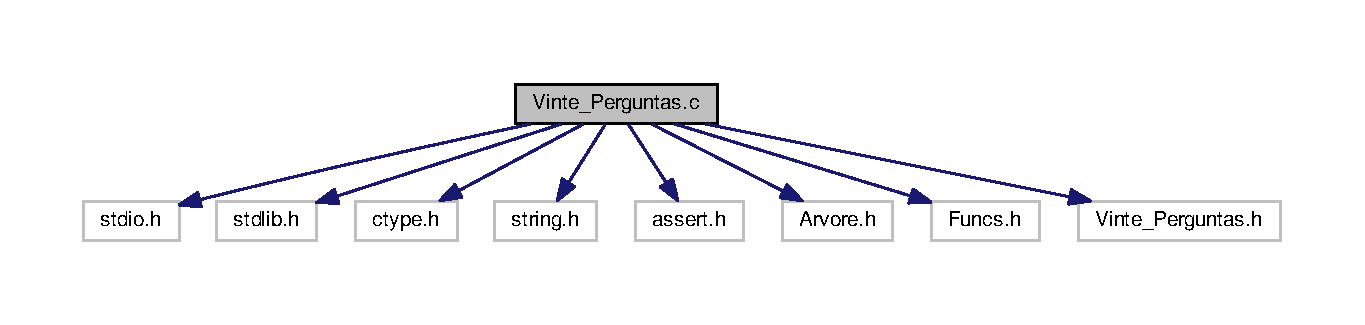
\includegraphics[width=350pt]{Vinte__Perguntas_8c__incl}
\end{center}
\end{figure}
\subsection*{Definições e Macros}
\begin{DoxyCompactItemize}
\item 
\#define \hyperlink{Vinte__Perguntas_8c_aa9c92c11eef6b6d98a1a444302093ca5}{\+\_\+\+Primary\+\_\+libraries}
\begin{DoxyCompactList}\small\item\em Header de funções padrão, para I/O, manipulação de strings. \end{DoxyCompactList}\item 
\#define \hyperlink{Vinte__Perguntas_8c_ad3059c7e862e1f571f036f8edbec268e}{\+\_\+\+Arvore\+\_\+library}\hypertarget{Vinte__Perguntas_8c_ad3059c7e862e1f571f036f8edbec268e}{}\label{Vinte__Perguntas_8c_ad3059c7e862e1f571f036f8edbec268e}

\begin{DoxyCompactList}\small\item\em Header da biblioteca de arvore. \end{DoxyCompactList}\item 
\#define \hyperlink{Vinte__Perguntas_8c_aada0c2263d9b6d55cbf5b649bc72a64a}{\+\_\+\+Funcs\+\_\+library}\hypertarget{Vinte__Perguntas_8c_aada0c2263d9b6d55cbf5b649bc72a64a}{}\label{Vinte__Perguntas_8c_aada0c2263d9b6d55cbf5b649bc72a64a}

\begin{DoxyCompactList}\small\item\em Header da biblioteca de funções (criação de arquivo e concatenação de strings). \end{DoxyCompactList}\item 
\#define \hyperlink{Vinte__Perguntas_8c_a18fc926bd99ef27d0302ea3f50e1424e}{\+\_\+\+Vinte\+\_\+\+Perguntas\+\_\+library}\hypertarget{Vinte__Perguntas_8c_a18fc926bd99ef27d0302ea3f50e1424e}{}\label{Vinte__Perguntas_8c_a18fc926bd99ef27d0302ea3f50e1424e}

\begin{DoxyCompactList}\small\item\em Header da biblioteca de estruturação (execução) do jogo de 20 perguntas. \end{DoxyCompactList}\end{DoxyCompactItemize}
\subsection*{Funções}
\begin{DoxyCompactItemize}
\item 
int \hyperlink{Vinte__Perguntas_8c_a750ed2de98e06946b1287d1fd3aeff08}{Resposta} (int tipo)
\begin{DoxyCompactList}\small\item\em Função para pegar o input especifico de opções do usuario. \end{DoxyCompactList}\item 
void \hyperlink{Vinte__Perguntas_8c_a50cd5030c633ddd0c6cc9bcfb9adfd88}{Vinte\+\_\+\+Perguntas} (arvore $\ast$$\ast$anavega, int numero\+\_\+respostas)
\begin{DoxyCompactList}\small\item\em Função de execução do programa. \end{DoxyCompactList}\item 
void \hyperlink{Vinte__Perguntas_8c_a843ac3fa2d2a9236370d2771e011fbde}{Pergunta\+\_\+\+Final} (arvore $\ast$$\ast$anterior, arvore $\ast$$\ast$ainicio, int numero\+\_\+respostas, int opcao)
\begin{DoxyCompactList}\small\item\em Função que verifica se o computador acertou o objeto, e cria mais perguntas caso não tenha acertado (se o usuário quiser e ainda não tenham sido respondidas 20 perguntas). \end{DoxyCompactList}\end{DoxyCompactItemize}


\subsection{Descrição Detalhada}
Arquivo que contem a biblioteca de estruturação (execução) do jogo de 20 perguntas. 

\begin{DoxyAuthor}{Autor}
Andre Garrido Damaceno 
\end{DoxyAuthor}


\subsection{Definições e macros}
\index{Vinte\+\_\+\+Perguntas.\+c@{Vinte\+\_\+\+Perguntas.\+c}!\+\_\+\+Primary\+\_\+libraries@{\+\_\+\+Primary\+\_\+libraries}}
\index{\+\_\+\+Primary\+\_\+libraries@{\+\_\+\+Primary\+\_\+libraries}!Vinte\+\_\+\+Perguntas.\+c@{Vinte\+\_\+\+Perguntas.\+c}}
\subsubsection[{\texorpdfstring{\+\_\+\+Primary\+\_\+libraries}{_Primary_libraries}}]{\setlength{\rightskip}{0pt plus 5cm}\#define \+\_\+\+Primary\+\_\+libraries}\hypertarget{Vinte__Perguntas_8c_aa9c92c11eef6b6d98a1a444302093ca5}{}\label{Vinte__Perguntas_8c_aa9c92c11eef6b6d98a1a444302093ca5}


Header de funções padrão, para I/O, manipulação de strings. 

Como esse arquivo contem a biblioteca de execução, necessita dos headers padrões, de funções auxiliares, e de estruturação do jogo. 

\subsection{Funções}
\index{Vinte\+\_\+\+Perguntas.\+c@{Vinte\+\_\+\+Perguntas.\+c}!Pergunta\+\_\+\+Final@{Pergunta\+\_\+\+Final}}
\index{Pergunta\+\_\+\+Final@{Pergunta\+\_\+\+Final}!Vinte\+\_\+\+Perguntas.\+c@{Vinte\+\_\+\+Perguntas.\+c}}
\subsubsection[{\texorpdfstring{Pergunta\+\_\+\+Final(arvore $\ast$$\ast$anterior, arvore $\ast$$\ast$ainicio, int numero\+\_\+respostas, int opcao)}{Pergunta_Final(arvore **anterior, arvore **ainicio, int numero_respostas, int opcao)}}]{\setlength{\rightskip}{0pt plus 5cm}void Pergunta\+\_\+\+Final (
\begin{DoxyParamCaption}
\item[{arvore $\ast$$\ast$}]{anterior, }
\item[{arvore $\ast$$\ast$}]{ainicio, }
\item[{int}]{numero\+\_\+respostas, }
\item[{int}]{opcao}
\end{DoxyParamCaption}
)}\hypertarget{Vinte__Perguntas_8c_a843ac3fa2d2a9236370d2771e011fbde}{}\label{Vinte__Perguntas_8c_a843ac3fa2d2a9236370d2771e011fbde}


Função que verifica se o computador acertou o objeto, e cria mais perguntas caso não tenha acertado (se o usuário quiser e ainda não tenham sido respondidas 20 perguntas). 

Essa função recebe como parametro o endereço do ponteiro da arvore \textquotesingle{}arvore $\ast$$\ast$anterior\textquotesingle{}, o endereço do apontador do inicio da arvore \textquotesingle{}arvore $\ast$$\ast$ainicio\textquotesingle{}, o numero de perguntas ja respondidas \textquotesingle{}int numero\+\_\+respostas\textquotesingle{} e a última opção selecionada \textquotesingle{}int opcao\textquotesingle{}. A função não retorna nenhum parametro. Essa função tem o objetivo de checar se o computador conseguiu chegar na resposta do objeto que o usuário pensava. Dessa forma, a função dá a opção de criar novas perguntas para alcançar esse objetivo (caso o usuário tenha respondido menos que 20 perguntas ou um nó foi apagado) e por fim, retorna ao jogo (ou mostra o resultado caso ja tenham sido respondidas as 20 perguntas). Os casos de erro são os mesmos das funções \textquotesingle{}\hyperlink{Vinte__Perguntas_8c_a50cd5030c633ddd0c6cc9bcfb9adfd88}{Vinte\+\_\+\+Perguntas()}\textquotesingle{} e \textquotesingle{}\hyperlink{Arvore_8c_a11bdc8462ac661708ec7dfc6209ad039}{Constroi\+\_\+\+Manual()}\textquotesingle{}, pois depende dessas funções e de alocação de memoria do computador, sendo assim, a execução é terminada caso haja algum erro de alocação. \index{Vinte\+\_\+\+Perguntas.\+c@{Vinte\+\_\+\+Perguntas.\+c}!Resposta@{Resposta}}
\index{Resposta@{Resposta}!Vinte\+\_\+\+Perguntas.\+c@{Vinte\+\_\+\+Perguntas.\+c}}
\subsubsection[{\texorpdfstring{Resposta(int tipo)}{Resposta(int tipo)}}]{\setlength{\rightskip}{0pt plus 5cm}int Resposta (
\begin{DoxyParamCaption}
\item[{int}]{tipo}
\end{DoxyParamCaption}
)}\hypertarget{Vinte__Perguntas_8c_a750ed2de98e06946b1287d1fd3aeff08}{}\label{Vinte__Perguntas_8c_a750ed2de98e06946b1287d1fd3aeff08}


Função para pegar o input especifico de opções do usuario. 

Essa função recebe como parametro um inteiro \textquotesingle{}int tipo\textquotesingle{}, que especifica o tipo de opção que o usuário terá e retorna um inteiro que representa a opção selecionada (escrita) pelo usuario. Essa função inicialmente lê a resposta escrita pelo usuário e delimita as respostas para o Tipo da pergunta, sendo \textquotesingle{}simples\textquotesingle{} -\/ para perguntas de \textquotesingle{}sim\textquotesingle{} ou \textquotesingle{}nao\textquotesingle{}, \textquotesingle{}multipla\textquotesingle{} -\/ para perguntas de \textquotesingle{}sim\textquotesingle{}, \textquotesingle{}nao\textquotesingle{}, \textquotesingle{}editar\textquotesingle{} ou \textquotesingle{}apagar\textquotesingle{}, e \textquotesingle{}inicializacao\textquotesingle{} -\/ para perguntas de \textquotesingle{}abrir\textquotesingle{} ou \textquotesingle{}criar\textquotesingle{}. Caso o usuario tenha respondido algo invalido, é mencionada as respostas que a pergunta espera, e dada a chance do usuario responder novamente, caso contrario, é retornado o equivalente da resposta do usuario pelo inteiro. Caso haja um erro de leitura pelo \textquotesingle{}scanf\textquotesingle{} (usuario digita mais que 6 caracteres), apenas é mencionada a mensagem dos tipos da resposta disponivel multiplas vezes, qualquer outro tipo de erro é desconhecido o comportamento (pois estariam dependendo das funções \textquotesingle{}strcmp\textquotesingle{}, \textquotesingle{}strlen\textquotesingle{} e toupper). \index{Vinte\+\_\+\+Perguntas.\+c@{Vinte\+\_\+\+Perguntas.\+c}!Vinte\+\_\+\+Perguntas@{Vinte\+\_\+\+Perguntas}}
\index{Vinte\+\_\+\+Perguntas@{Vinte\+\_\+\+Perguntas}!Vinte\+\_\+\+Perguntas.\+c@{Vinte\+\_\+\+Perguntas.\+c}}
\subsubsection[{\texorpdfstring{Vinte\+\_\+\+Perguntas(arvore $\ast$$\ast$anavega, int numero\+\_\+respostas)}{Vinte_Perguntas(arvore **anavega, int numero_respostas)}}]{\setlength{\rightskip}{0pt plus 5cm}void Vinte\+\_\+\+Perguntas (
\begin{DoxyParamCaption}
\item[{arvore $\ast$$\ast$}]{anavega, }
\item[{int}]{numero\+\_\+respostas}
\end{DoxyParamCaption}
)}\hypertarget{Vinte__Perguntas_8c_a50cd5030c633ddd0c6cc9bcfb9adfd88}{}\label{Vinte__Perguntas_8c_a50cd5030c633ddd0c6cc9bcfb9adfd88}


Função de execução do programa. 

Essa função recebe como parametro o endereço do ponteiro da arvore \textquotesingle{}arvore $\ast$$\ast$anavega\textquotesingle{} (para as possiveis mudanças na arvore como apagar, editar, navegar e criar novos nós) e um inteiro \textquotesingle{}int numero\+\_\+respostas\textquotesingle{}, para saber quantas perguntas ja foram respondidas pelo usuario. Essa função não retorna nenhum parametro. A função inicialmente alerta ao usuário que o jogo irá começar e analisa se a arvore é vazia ou o numero\+\_\+respostas é menor que 19 (ja foram respondidas 20 perguntas). Em seguida é lida a pergunta para o usuário e ele pode navegar pelas perguntas (respondendo \textquotesingle{}sim\textquotesingle{} ou \textquotesingle{}nao\textquotesingle{}) ou editar/apagar uma pergunta. No fim, é perguntado ao usuário se seu objeto pensado foi descoberto. Caso tenha sido, o jogo é finalizado, caso não tenha sido e o usuário ainda não tenha respondido 20 perguntas, é perguntado se o usuário deseja inserir mais perguntas para o programa descobrir o objeto. Ao fim das inserções, o jogo recomeça a partir do ponto da ultima pergunta respondida pelo usuário. Como essa função de execução utiliza a maior parte de todas as funções criadas, os erros estão relacionados a essas funções. Mas todas as funções inclusive essa, foi desenvolvida para conter erros e finalizar o programa apenas se um erro de alocação de memoria ocorrer. 
%--- End generated contents ---

% Index
\backmatter
\newpage
\phantomsection
\clearemptydoublepage
\addcontentsline{toc}{chapter}{Índice}
\printindex

\end{document}
